\documentclass[12pt,a4paper]{article}
\usepackage{amsmath,amssymb,amsthm}
\usepackage[margin=2.5cm]{geometry}
\usepackage{booktabs}
\usepackage{enumitem}
\usepackage{hyperref}
\hypersetup{
  hidelinks,
  pdftitle={Physics from Existence I: The Equation},
  pdfauthor={Hidekazu Kondo},
  pdfsubject={Physics from Existence},
  pdfkeywords={physics, Standard Model, information geometry, entropy, existence}
}
\usepackage{needspace}
\usepackage{graphicx}
\graphicspath{{supplementary/}}

\newtheorem{theorem}{Theorem}
\newtheorem{proposition}{Proposition}
\newtheorem{corollary}{Corollary}
\newtheorem{remark}{Remark}

% Paper II mark (rigorisation of the flagged claim is given in Paper II; declared once in §1)
\newcommand{\PII}{\textsuperscript{\textup{II}}}

\title{\textbf{Physics from Existence I: The Equation}\\[0.45em]{\large The Binary-Entropy Equation $V = -H$ and the Structure of Standard-Model Parameters}}
\author{Hidekazu Kondo\\ \textit{Tokyo, Japan}}
\date{April 2026}

\begin{document}
\maketitle

\begin{abstract}\sloppy
No theory has simultaneously derived all 26 free parameters
of the Standard Model.
In this paper, we show that three axioms about existence---existence is bivalent ($n \in \{0,1\}$, i.e.\ $n^2{=}n$), existence is uncertain ($\sigma{\neq}1$), and non-existence is forbidden ($\sigma{\neq}0$)---uniquely determine the single equation $V = -H$ as an algebraic identity. The mathematical structure generated by this equation corresponds to that of the Standard Model, reproducing more than 20 physical quantities with no adjustable parameters, all agreeing with experiment to $0.0006\%$--$2.6\%$ accuracy.

$V = -H$ is the canonical free energy of a single binary degree of freedom
$n \in \{0,1\}$, determined as the Legendre transform
of the Fermi--Dirac distribution.
The Schr\"odinger equation is derived as a transfer matrix from this potential and the kinetic term of the canonical normalisation ($g=1$, \S2.4).
This equation has exactly three bound states (discrete solutions),
corresponding to the three generations of fermions.
The spatial dimension $d = 3$ follows from three
conditions---preservation of the well, spin-statistics, and propagating gravity.
The mathematical structure unfolding from this coincidence
reproduces the gauge group
$\mathrm{SU}(3){\times}\mathrm{SU}(2){\times}\mathrm{U}(1)$.

More than 20 physical constants are derived from this
structure, including
$1/\alpha = 137.0368$ ($0.0006\%$),
$\alpha_s = 0.1179$ ($0.01\%$),
$\sin^2\!\theta_W = 3/13$ ($0.2\%$),
the charged-lepton mass ratio $R = 1.5293$ ($0.006\%$), and
$\sin\theta_C = 0.2245$ ($0.10\%$).
The results further predict the absolute neutrino masses ($\Sigma m_\nu = 59.2$~meV) and strictly zero neutrinoless double-beta decay, yielding seven testable predictions.
These quantities are not independent input
parameters---they are all computed from the same
mathematical structure fixed by $V = -H$.
\end{abstract}


%=====================================================================
\section{Introduction}
%=====================================================================

The Standard Model is the most successful theory of particle physics.
It describes all known particle interactions and has withstood
extensive experimental tests, including the discovery of the Higgs boson~\cite{atlas,cms} (2012).
Yet the theory contains
26 free parameters\footnote{The minimal Standard Model with massless
neutrinos has 19 free parameters~\cite{pdg}; adding three neutrino
masses and four PMNS parameters gives 26.
Some references count 25, absorbing $v_\mathrm{EW}$ into the
energy scale.}---fermion masses (Yukawa couplings),
mixing angles, gauge couplings, the Higgs self-coupling, and CP phases.
Their values must be measured and input by hand;
why they take those values is not explained within the Standard Model.
The generation number $N = 3$ is likewise an unexplained input.
Despite many attempts---grand unified theories (GUTs), supersymmetry (SUSY),
string theory---no theory has simultaneously determined all 26 parameters
with zero free parameters~\cite{xing}.
Even a single constant, the fine-structure constant~$\alpha$, has a long
history of attempts at first-principles
derivation~\cite{eddington,wyler,jentschura}, but these have remained isolated
numerical coincidences, lacking a unifying equation or mechanism.

An alternative approach seeks to derive physics from information theory.
Wheeler's ``it from bit''~\cite{wheeler} proposed that physical reality
arises from information but lacked a mathematical framework.
Jaynes~\cite{jaynes} derived statistical mechanics from entropy maximization
but did not reach quantum field theory.
Verlinde~\cite{verlinde} derived gravitational force from entropic reasoning
but addressed gravity alone.
Other approaches include Frieden's~\cite{frieden} Fisher information,
Caticha's~\cite{caticha} information geometry, and the informational
axiomatisations of Hardy~\cite{hardy} and Chiribella
et~al.~\cite{chiribella}.
All of these approaches share a common limitation:
they derive the \emph{form} of physical equations but not the
\emph{values} of the constants that appear in them. The closest published programme in spirit is the spectral Standard Model of Connes and Chamseddine~\cite{connes96,chamconnes96,ccm07}, which derives the SM gauge group, Higgs sector, and parameter relations from a noncommutative-geometric structure; its parameter-free prediction $m_H \approx 170$~GeV was falsified and later repaired by adding a singlet field---a direct cautionary precedent for parameter-free mass predictions, to which the predictions of this paper are equally subject. A related algebraic reconstruction is Furey's division-algebra approach~\cite{furey}.

This paper starts from three axioms:
Existence ($n \in \{0,1\}$), Uncertainty ($\sigma \neq 1$),
and Non-existence is forbidden ($\sigma \neq 0$).
Together A2 and A3 determine $\sigma \in (0,1)$, a partition function
$Z = 1 + e^\phi$, and, via the Legendre transform of the
Fermi--Dirac distribution, the canonical free energy
$V = -H(\sigma(\phi))$ as an algebraic identity,
where $H$ is the binary Shannon entropy,
$\sigma(\phi)$ is the Fermi--Dirac distribution (sigmoid function),
and $\phi = \operatorname{logit}(\sigma)$ is the natural
parameter~\cite{amari,ay}.
The Schr\"odinger equation is derived as a transfer matrix from this potential and the kinetic term of the canonical normalisation ($g=1$, \S2.4).

This Schr\"odinger equation has exactly three
bound states ($N = 3$), corresponding to the three generations
of fermions.
The spatial dimension $d_\mathrm{space} = 3$ follows from
three conditions---preservation of the well, spin-statistics, and propagating gravity;
the spacetime dimension $D = 4$ follows from gravitational degree-of-freedom matching and $\mathbb{C}P^2$, and the signature $(3,1)$ follows as a connection to the $M_2(\mathbb{C})_{sa}$ carrier structure (\S4, \S\ref{sec:4d}).
The gauge structure $\mathrm{PG}(2,\mathbb{F}_3)$
emerges from the coincidence $N = d = 3$,
corresponding uniquely to the gauge group
$\mathrm{SU}(3){\times}\mathrm{SU}(2){\times}\mathrm{U}(1)$.
From the representations of this gauge group,
a structure yielding 48~fermions, 12~gauge bosons, and 1~Higgs
is derived (\S\ref{sec:gauge}).
More than 20 parameters are derived---including
$1/\alpha_\mathrm{em} = 137.0368$ ($0.0006\%$),
$\sin^2\!\theta_W = 3/13$ ($0.2\%$),
the charged-lepton mass ratio $R = 1.5293$ ($0.006\%$),
Koide's $Q \approx 3/2$ ($\delta = -1.5 \times 10^{-5}$),
and CKM and PMNS mixing angles---all
at $0.0006\%$--$2.6\%$ accuracy with zero adjustable parameters
(\S\ref{sec:results}).
The associated Paper~II reconstruction additionally gives the
matching-point condition $\bar\theta(\mu_0)=0$\PII{}; it is not a
consequence of $V$-parity alone.

Beyond the numerical agreement, the mathematical structure derived from $V = -H$ corresponds to structural problems of the Standard Model. The role played in the Standard Model by $\mu^2 > 0$---moving the vacuum from the symmetric point to a finite field value---is played here by the shape of the well of $V$ (\S\ref{sec:higgs}); the bounded internal potential ($V \in [-\ln 2, 0]$) supplies no instability channel, so neither the metastability problem nor the hierarchy problem arises within this construction (the correspondence to 4D vacuum stability and the hierarchy problem requires the reconstruction matching). Since $V = -H$ is uniquely determined as the canonical free energy of $n \in \{0,1\}$, the Higgs is fixed to be unique.

This paper shows that, when the mathematical structure generated by $V = -H$ is placed in correspondence with the structure of the Standard Model, the resulting numerical values agree with experiment; it does not claim to derive the Standard Model itself rigorously from first principles. Moreover, at various points choices arise that the expansion of the equation alone does not determine — which fraction, operator, or coefficient of the structure reads off each observable. This paper states each such choice (a readout specification) explicitly and computes the values. That these choices are not free parameters — the proof of their uniqueness and rigidity — together with the operator-level derivations of the individual constructions in this paper, is given in Paper~II~\cite{paper2}; we do not repeat this attribution at each occurrence.

The paper is organized as follows.
Section~\ref{sec:chain} derives $V = -H$ from three axioms
and establishes the Schr\"odinger equation.
Section~\ref{sec:theorem} proves the bound-state count $N = 3$
as a mathematical theorem.
Section~\ref{sec:dimension} derives the spatial dimension $d = 3$
as the unique common solution of three independent realisation-consistency conditions.
Section~\ref{sec:gauge} constructs the gauge structure from
$\mathrm{PG}(2,\mathbb{F}_3)$.
Section~\ref{sec:couplings} derives the gauge coupling constants.
Section~\ref{sec:higgs} derives the Higgs mass and shows that the vacuum is pinned at an interior point with the internal potential bounded (no instability channel).
Section~\ref{sec:physics} places the bound states in correspondence with the three generations of charged leptons and derives fermion masses and mixing.
Section~\ref{sec:4d} confirms the spacetime dimension $D = 4$ and signature $(3,1)$ by consistency checks with stated premises, and establishes the tensor-product structure $\mathcal{H}_\mathrm{int}(\phi) \otimes \mathcal{H}_\mathrm{space}(x)$ from the independence of the construction.
Section~\ref{sec:results} summarises all results and
presents falsifiable predictions.
Section~\ref{sec:conclusion} gives the conclusion.


%=====================================================================
\section{From Existence to the Equation}\label{sec:chain}
%=====================================================================

This chapter formalises three axioms about existence mathematically
and derives the fundamental equation $V = -H$ through an algebraic
transformation.
From this equation, a structure consistent with the Standard Model emerges.

\subsection{The Axioms}

We define the three axioms on which the entire structure of this
paper rests.

\noindent\textbf{A1~(Existence):}\;
Something exists. ``Exists'' is a proposition; it is either true
or false --- by the law of excluded middle, there is no third value.
Writing the state of existence as~$n$, the state space is
$n \in \{0,1\}$. A1 defines the state space but does not
determine the \textbf{value} of~$n$.

\medskip
\noindent\textbf{A2~(Uncertainty):}\;
Existence is uncertain. Whatever exists does not exist with
certainty: the occupation probability
$\sigma = \langle n \rangle$ satisfies $\sigma \neq 1$.
A2 excludes the upper endpoint (certain existence) but says nothing
about the lower endpoint.

\medskip
\noindent\textbf{A3~(Prohibition of non-existence):}\;
Non-existence is not a state ($\sigma \neq 0$). A way of being
that consists in not-being is a contradiction.

\medskip
\noindent
From these three axioms, the structure and constants of the
Standard Model follow. We now formalise them.


\subsection{Bivalence and the Partition Function}\label{sec:partition}

Starting from the state space $n \in \{0,1\}$ established by A1,
we construct the partition function.

Since $n$ takes only the values 0 and~1,
\begin{equation}\label{eq:idempotency}
  n^2 = n
\end{equation}
follows --- because the solutions of $n(n{-}1) = 0$ are exactly
$\{0,1\}$. However, A1 alone leaves the system in a pure state
$n = 0$ or $n = 1$, with no dynamics.
A2 ($\sigma \neq 1$) excludes certain existence;
A3 ($\sigma \neq 0$) excludes non-existence.
Together they determine $\sigma \in (0,1)$:
the system is described as a canonical ensemble of a binary
variable---an exponential family with mean parameter $\sigma$---neither
certainly present nor certainly absent. The tilt weight $e^{n\phi}$ has its tilt coefficient fixed to~1 (generation-normalisation rigidity)\PII{}.
$n^2 = n$ truncates the sum to two terms, and the partition
function is
\begin{equation}
  Z = \sum_{n=0}^{1} e^{n\phi} = 1 + e^{\phi},
\end{equation}
where $\phi = \ln[\sigma/(1{-}\sigma)]$ (the logit transform) is
the canonical coordinate of the exponential family. Were $n$ able to take values $0, 1, 2, \dots$ (Bose statistics), the sum would be an infinite series. As a consequence of the law of excluded middle, $n^2 = n$ forbids this and restricts the occupation number to $\{0,1\}$---the Fermi--Dirac occupation statistics. Exchange antisymmetry (spin statistics) does not follow from this alone; it is carried by the many-body realisation (\S5.2).

The expectation
$\sigma = \langle n \rangle = \partial\ln Z/\partial\phi$
coincides with the Fermi--Dirac distribution, and its variance is
the source of all subsequent structure:
\begin{equation}
  \sigma = \frac{1}{1+e^{-\phi}}, \qquad
  g_F = \sigma(1{-}\sigma) = \mathrm{Var}(n) > 0.
\end{equation}
These are not assumed but derived, from the combination of A1
(bivalence), A2 (uncertainty: $\sigma \neq 1$),
and A3 (non-existence forbidden: $\sigma \neq 0$). $g_F$ is the gap between the
binary observable ($n^2 = n$) and its uncertain expectation
($\sigma^2 \neq \sigma$), and vanishes only at the pure values
$\sigma \in \{0,1\}$.


\subsection{The Effective Potential \texorpdfstring{$V = -H$}{V = -H}}

\S2.2 established the partition function $Z = 1+e^\phi$.
The next step is to construct an effective potential from it.

The naive choice $-\ln Z$ diverges as
$\phi \to \infty$, so a Legendre transform to the canonical
free energy is required.
The logarithm $W = \ln Z$ of the partition function
generates the classical field
$\sigma = dW/d\phi$ and yields the effective potential:
\begin{equation}\label{eq:legendre}
  V(\phi) = \phi\sigma - W(\phi)
  = \sigma\ln\sigma + (1{-}\sigma)\ln(1{-}\sigma) = -H(\sigma),
\end{equation}
where $H(p) = -p\ln p - (1{-}p)\ln(1{-}p)$
is binary Shannon entropy~\cite{shannon}.

That is, $V = -H$ is an algebraic identity:
the canonical free energy of a single binary degree of freedom
$n \in \{0,1\}$ equals the negative of the Shannon entropy.
There is no freedom of choice.
The potential
\begin{equation}\label{eq:VH}
  V = -H
\end{equation}
is thereby uniquely determined by axioms A1--A3 together with the
exponential-family realisation above.
From this single equation, a structure closely matching
the Standard Model emerges, and values agreeing with physical
constants to high precision are derived (\S3--\S10).


\subsection{The Schr\"odinger Equation}\label{sec:kinetic}

\S2.3 established $V = -H$ as the potential. The next question is how many discrete states this potential well can hold. To answer it, an eigenvalue equation is needed, which requires a kinetic term in addition to the potential. The kinetic term likewise follows from the same structure (its relative normalisation is fixed by $g = 1$ below).

The exponential family of a binary variable has two natural flat coordinates: $u = 2\arcsin\sqrt{\sigma}$, in which the Fisher metric is flat, and $\phi = \mathrm{logit}(\sigma)$, in which the e-connection is flat~\cite{cencov,amari,ay}. A3 forbids $\sigma = 0$. The coordinate $u$ places $\sigma = 0$ at the finite point $u = 0$, so defining the dynamics requires boundary-condition data at that point---the point of non-existence becomes a repository of model-defining data. The coordinate $\phi$ sends $\sigma = 0$ to $\phi \to -\infty$ and requires no boundary data. A3 therefore selects~$\phi$. Free motion on the e-flat coordinate~$\phi$ has a Lagrangian that is a constant-coefficient quadratic form in $\dot{\phi}$.

The choice of $\phi$ fixes the coordinate, but not the relative normalisation of the kinetic term and the action weight. Writing the kinetic coefficient as $a^2/2$ and the action weight as $b$ (the family $-(a^2/2)\,d^2\!/d\phi^2 - b\,H(\sigma(\phi))$), the remaining freedom is the single dimensionless ratio $g = b/a^2$. The scale of $\phi$ is fixed by the binary indicator of A1, the scale of $V = -H$ by the Legendre identity, and rescaling the step size changes $a^2$ and $b$ in the same proportion, leaving $g$ unchanged. This paper adopts the canonical normalisation $g = 1$, which measures the quadratic variation per step of $\phi$ and the action weight as quantities of the same transfer process.\PII{} The Landauer viewpoint supports the same normalisation: with $\phi$ as the e-affine coordinate, the transfer kernel takes the form $K(\phi', \phi; \Delta\tau) \propto \exp[-(\phi'-\phi)^2/(2\Delta\tau) - \Delta\tau V(\phi)]$, and fixing the information metric per bit to unity gives kinetic coefficient 1, consistent with $g = 1$ (an independent corroboration).

These choices---the canonicity of the coordinate (any coordinate linearising the tilting action is unique up to affine maps), the constancy of the kinetic coefficient (homogeneity under displacement excludes position-dependent coefficients), and the exclusion of $u$-type coordinates (which have reachable boundaries)---are established as rigidity theorems\PII{}. The bound-state count $N = 3$ is invariant across the family $-\tfrac{1}{2}\,d^2\!/d\phi^2 - g\,H(\sigma(\phi))$ for $g \in [0.80, 1.50]$ (verified pointwise; certificate included). This robustness concerns the count $N$ only: $\varepsilon = N - \sqrt{g}\,n_\mathrm{WKB}(1)$ changes sign within the same window ($+0.51$ at $g = 0.80$, $-0.41$ at $g = 1.50$), so all $\varepsilon$-dependent corrections of \S6--\S8 rely on $g = 1$ being fixed (the rigidity theorems above). At the lower edge $g = 0.80$ the action count $2.49$ falls slightly below the third-state Maslov threshold $2.5$ while the exact count remains $3$---an instance showing that the threshold rule of \S3.1 is only a heuristic.

Combining $V = -H$ as the potential with the kinetic term of the canonical normalisation ($g = 1$):
\begin{equation}\label{eq:schrodinger}
  \left[-\frac{1}{2}\frac{d^2}{d\phi^2} - H(\sigma(\phi))\right]\Psi = E\,\Psi
\end{equation}
\noindent
This is nothing other than a Schr\"odinger equation: with only the three axioms of existence and the canonical normalisation $g = 1$ above as input, the eigenvalue equation of quantum mechanics emerges as the continuum limit of the transfer matrix of the canonical action.

The bound-state count $N = 3$ is a consequence of this construction---the A3-selected coordinate $\phi$ together with a flat kinetic term. Writing the flat kinetic term in a different coordinate yields a different operator and a different spectrum, so the A3 selection of $\phi$ is essential.

The derivation chain of \S2 is summarised as:
\[
\begin{gathered}
  \text{A1--A3}\;\Rightarrow\; n^2{=}n,\; 0<\sigma<1
  \;\Rightarrow\; Z = 1{+}e^{\phi}
  \;\xrightarrow{\text{Legendre}}\; V = -H\\
  \;\xrightarrow{\text{transfer matrix}}\;
  \left[-\tfrac{1}{2}\partial_\phi^2 + V\right]\Psi = E\Psi
\end{gathered}
\]


%=====================================================================
\section{Three Bound States}\label{sec:theorem}
%=====================================================================

Why do fermions come in exactly three generations---why $\tau$, $\mu$, $e$,
and why not a fourth?
This chapter proves that the potential $V = -H$ has exactly three
bound states (hereafter $N = 3$), and shows that this structurally
corresponds to the three generations of fermions.

\subsection{Why \texorpdfstring{$N = 3$}{N = 3}}\label{sec:whyN3}

The potential $V = -H$ is a well. It is deepest at the centre
($\phi = 0$) where $V = -\ln 2$,
returning to zero at both ends $\phi \to \pm\infty$.
In quantum mechanics, such a well confines discrete energy levels---by
the same principle that the hydrogen atom confines electrons to discrete
orbitals. A deep, wide well holds many levels; a shallow, narrow well
holds few. The well of $V = -H$ is shallow---its depth is only
$\ln 2 \approx 0.693$, and its shape is entirely determined by the
Shannon entropy.

\begin{figure}[ht]
\centering
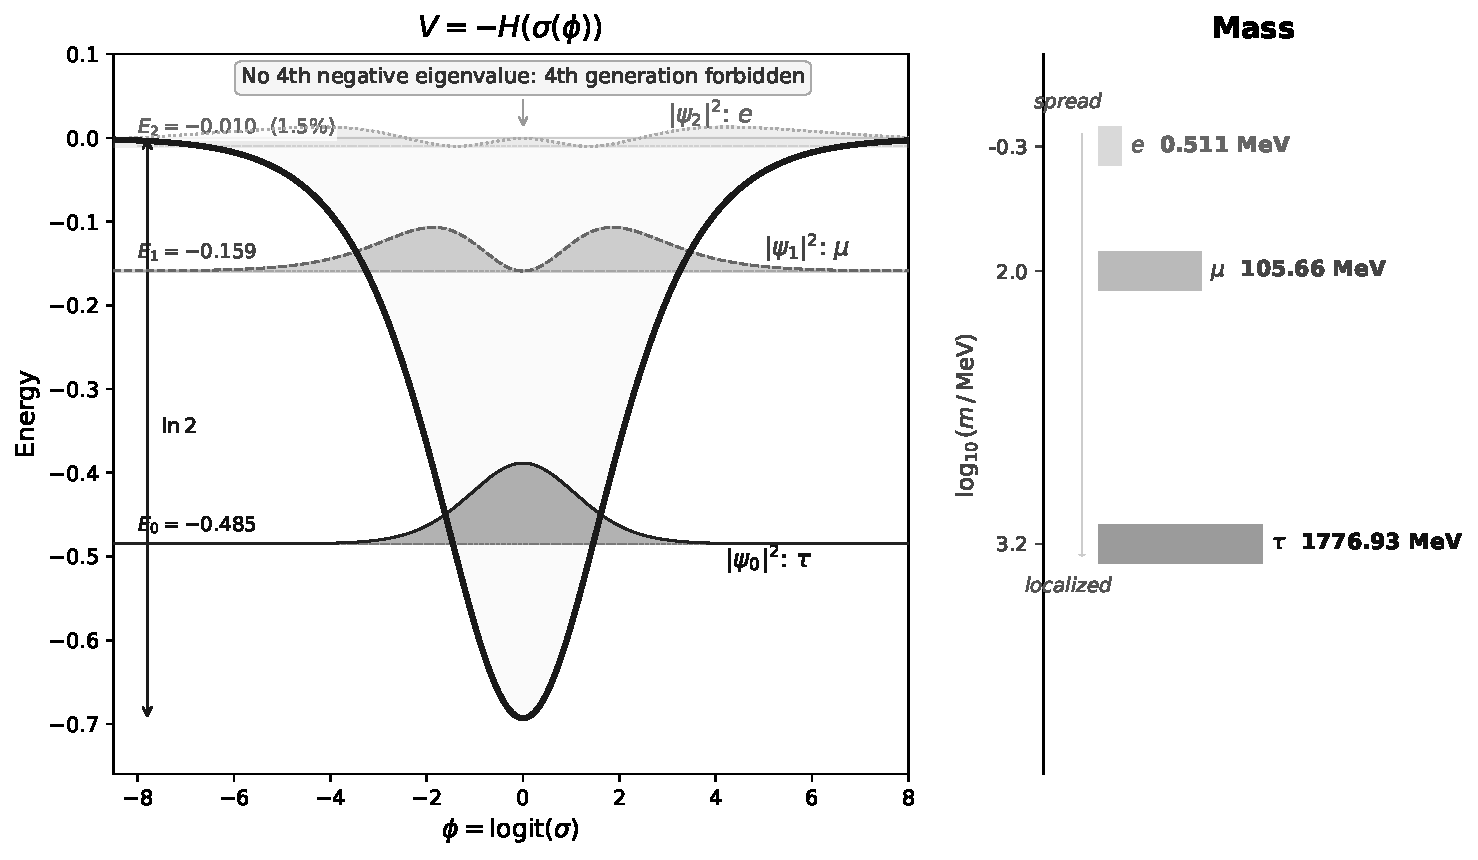
\includegraphics[width=\textwidth]{fig_potential.pdf}
\caption{The potential $V = -H(\sigma(\phi))$ and the probability
densities $|\psi_n|^2$ of its three bound states (left).
More localised states correspond to heavier particles (right).
No fourth negative eigenvalue: a fourth generation is forbidden.}
\label{fig:potential}
\end{figure}

We denote the number of levels confined in this well by~$N$.
A semiclassical (WKB) approximation estimates how many
half-wavelengths fit inside the well.
Each integer half-wavelength corresponds to one bound state:
\begin{equation}
  n_\mathrm{WKB}
  = \frac{1}{\pi}\int_{-\infty}^{\infty}
    \sqrt{2H(\sigma(\phi))}\,d\phi
  = 2.781\,.
\end{equation}
In the standard convention including the Maslov correction, the threshold for the $k$-th state is $n_\mathrm{WKB} > k - 1/2$. The value $n_\mathrm{WKB} = 2.781$ exceeds the third-state threshold $2.5$ by $0.281$, while falling short of the fourth-state threshold $3.5$ by $0.719$. The WKB estimate therefore suggests $N = 3$.
We define $\varepsilon \equiv N - n_\mathrm{WKB} = 3 - 2.781 = 0.219$, the gap between the exact bound-state count and this semiclassical action count.\footnote{The rigorous interval enclosure 0.219188 is given in Paper~II.} $\varepsilon > 0$ reflects the fact that the third state is barely bound. The numerical measure of how marginal it is depends on the semiclassical convention: measured against the Maslov-corrected threshold, the same gap is $2.781 - 2.5 = 0.281$. The expansion parameter of this paper is consistently this $\varepsilon$; it controls the NLO corrections to the couplings and mixing angles derived in \S6--\S8.
$N = 3$ arises from a construction of three elements---the choice of coordinate, the normalisation of the kinetic term, and the type of entropy. First, the coordinate $\phi = \mathrm{logit}(\sigma)$ is unique up to affine transformations as the coordinate linearising the tilt action, with its scale fixed by the binary indicator of A1 (\S2.4). Second, the kinetic-term normalisation is the canonical normalisation $g = 1$ of \S2.4. Third, Shannon entropy is the unique entropy satisfying the Khinchin axioms, which include strong additivity (the chain rule) (Khinchin's theorem~\cite{aczel,khinchin}). Under this construction, $N = 3$ is rigorously proved by interval arithmetic (\S\ref{sec:rigorous}).

\subsection{Rigorous Proof}\label{sec:rigorous}

\begin{theorem}[$N = 3$]\label{thm:N3}
The Schr\"odinger equation of \S2 has exactly three bound states, and their eigenvalues are rigorously enclosed by interval arithmetic:
\[
\begin{aligned}
  E_0 &= -0.4850022531029642374452777658 \pm 10^{-24},\\
  E_1 &= -0.1590522216188561779934190 \pm 10^{-24},\\
  E_2 &= -0.010423393062109459327616 \pm 10^{-22}
\end{aligned}
\]
No fourth negative eigenvalue exists; the essential spectrum begins at 0 (the small positive values seen on finite grids are discretisation artifacts of the box).
\end{theorem}

\noindent\textit{Proof (computer-assisted, interval arithmetic).}\;
By parity, decompose into the Neumann problem (even) and the Dirichlet problem (odd) on the half-line $[0,\infty)$. Under interval enclosures based on the monotonicity of the potential, propagate the Pr\"ufer angle by intervals and combine with analytic tail estimates to obtain rigorous upper and lower bounds on the Pr\"ufer angle at the trial energies. By Sturm oscillation theory, the number of negative eigenvalues is counted exactly by the rotation of the Pr\"ufer angle, giving exactly 2 in the even sector and exactly 1 in the odd sector---$N = 3$ in total. The eigenvalue enclosures are certified by two-sided shooting with a verified high-order Taylor integrator over interval coefficients. An independent implementation (Arb ball arithmetic) re-certifies the bound-state count $N = 3$. The bundled verification code additionally confirms the existence of three negative eigenvalues by variational upper bounds from Rayleigh quotients of three sech-type (Pöschl--Teller-type~\cite{poschl}) trial functions. Three certificate scripts are included in the supplementary materials.\hfill$\square$

\medskip\noindent
\textbf{Correspondence with generations.}
These three bound states $\psi_0$, $\psi_1$, $\psi_2$ correspond
to the three generations of fermions.
The ordering of binding energies $|E_0| > |E_1| > |E_2|$ corresponds
to the ordering of wavefunction localisation --- the most deeply
bound $\psi_0$ is the most localised at the centre of the well,
while the marginally bound $\psi_2$ is the most spread out.
As shown in \S\ref{sec:physics}, this localisation corresponds to mass,
and $\psi_0$, $\psi_1$, $\psi_2$ correspond to the heaviest through the lightest generation (for charged leptons, $\tau$, $\mu$, $e$).
The number of bound states~(3) and their ordering structure correspond
to the number of generations and the mass hierarchy.
The absence of a fourth negative eigenvalue predicts that a fourth generation does not exist.
The quantitative derivation of mass ratios and mixing angles is given
in \S\ref{sec:physics}.


%=====================================================================
\section{Three Spatial Dimensions}\label{sec:dimension}
%=====================================================================

Section~\ref{sec:theorem} proved $N = 3$.
The next question is:
if the mathematical structure of these three bound states
corresponds to physical structure, in how many spatial dimensions
can they be realised?
We now examine this.

Consider the same well shape $V = -H$ realised as a radial profile
in $d$-dimensional space.
Here $\sigma(r)$ is the same well shape as $\sigma(\phi)$ on $\phi \in \mathbb{R}$,
transferred to the radial variable $r \geq 0$; the difference in domain is
addressed below in the comparison with full-line quantisation.
Reducing the $d$-dimensional Schr\"odinger equation to a
one-dimensional radial equation by standard partial-wave
decomposition, an additional effective force
$(d{-}1)(d{-}3)/(8r^2)$ appears:
\begin{equation}
  V_\mathrm{eff}(r) = -H(\sigma(r))
    + \frac{(d{-}1)(d{-}3)}{8r^2}.
\end{equation}
The numerator $(d{-}1)(d{-}3)$ vanishes for $d = 1$ and $d = 3$,
leaving $V = -H$ unchanged.
In other dimensions, this geometric term deforms the operator:

\begin{center}\small
\begin{tabular}{ccc}
\toprule
$d$ & $(d{-}1)(d{-}3)/8$ & Effect on the operator \\
\midrule
1 & 0 & No deformation \\
2 & $-1/8$ & Attractive term (tends to create extra states) \\
3 & \textbf{0} & \textbf{No deformation: the well shape is preserved} \\
4 & $+3/8$ & Repulsive term (tends to remove the marginal third state) \\
$\geq 5$ & $\geq 1$ & Strong repulsion \\
\bottomrule
\end{tabular}
\end{center}

\noindent
Full-line quantisation ($\phi \in \mathbb{R}$) is essentially self-adjoint at the endpoints and requires no boundary condition. Under A3 (non-existence is not a state---no additional data is admissible at the boundary)\PII{}, this canonical full-line quantisation is the reference, and a spatial realisation is required not to add an extra inverse-square term to the canonical operator. This requirement is met only when the coefficient $(d{-}1)(d{-}3)/8$ vanishes, i.e.\ only for $d = 1, 3$. Note that a vanishing inverse-square term does not make the full-line and radial problems identical---a half-line radial model adds endpoint structure at the origin (a choice of self-adjoint extension) and is a different model, outside the comparison fixed by this correspondence (Paper~II).

Two realisation-consistency conditions exclude $d = 1$.
First, the fermionic structure (CAR) is derived from A1--A3
(base-independent bivalence)\PII{}; the half-integer spin its
spatial realisation requires holds by the spin-statistics theorem
for $d \geq 3$
($\pi_1(\mathrm{SO}(d)) = \mathbb{Z}_2$, giving the double cover
$\mathrm{Spin}(d)$ with finite-dimensional spinor
representations).
Second, the realisation of a spin-2 field (gravity)---taken as a
premise, as in \S9.1, with its derivation left to a subsequent
paper---propagating dynamically requires $d \geq 3$ (for $d \leq 2$
the Weyl tensor vanishes identically, leaving no local degrees of
freedom).

We summarise this as a theorem.

\begin{theorem}[$d = 3$]\label{thm:d3}
Under the A3 selection of full-line quantisation, $d = 3$ is the unique spatial dimension simultaneously satisfying:
\emph{(i)}~the well operator is preserved with no extra geometric term: $d = 1, 3$;
\emph{(ii)}~spin-statistics connection holds: $d \geq 3$;
\emph{(iii)}~gravity propagates (Weyl tensor non-trivial): $d \geq 3$.
Intersection: $\{3\}$.
\end{theorem}

\noindent\textit{Proof.}\;
(i)~centrifugal term $(d{-}1)(d{-}3)/(8r^2) = 0$ iff $d = 1$ or $3$;
(ii)~$\pi_1(\mathrm{SO}(d)) = \mathbb{Z}_2$ for $d \geq 3$;
(iii)~the Weyl tensor vanishes identically in spacetime dimension
$\leq 3$, i.e.\ spatial $d \leq 2$; propagating gravity requires $d \geq 3$.\hfill$\square$


%=====================================================================

%=====================================================================
\section{Gauge Structure from the Projective Plane}\label{sec:gauge}
%=====================================================================

The generation number $N = 3$ (\S\ref{sec:theorem}) and the spatial
dimension $d = 3$ (\S\ref{sec:dimension}) were derived
independently---yet they take the same value $N = d = 3$.
On this coincidence, we construct the three-dimensional space $\mathbb{F}_3^3$ over the field $\mathbb{F}_3$.
This chapter shows that the geometric structure arising from it has the same
mathematical construction as the Standard Model gauge structure.

\subsection{Origin of the Gauge Structure}\label{sec:gauge-origin}

What gauge structure arises from $N = d = 3$?
The key is the fundamental difference between generations
and colour.

Quark colours (red, green, blue) are degenerate---every colour
has the same energy, so there is no preferred basis.
This equivalence generates the continuous rotation symmetry
$\mathrm{SU}(3)$.
Generations are different.
The three bound states of $V = -H$ all have distinct energies
($E_0 \neq E_1 \neq E_2$, by the Sturm--Liouville theorem),
so a preferred eigenbasis exists.
The symmetry preserving this basis is discrete and, as a gauge symmetry, cannot support a continuous group.\footnote{The $2C_F$ appearing in the mass readout of \S8.1 is the internal-localisation Casimir of $N = 3$ and is compatible with this.}

\S3 derived $N = 3$ (bound states) and \S4 derived $d = 3$
(spatial dimension).
From this coincidence, the three-dimensional space
$\mathbb{F}_3^3$ over the field $\mathbb{F}_3 = \{0,1,2\}$
is determined.
The projective construction that follows requires a field
(not merely a group); since $N = 3$ is prime,
$\mathbb{F}_3 = \mathbb{Z}/3\mathbb{Z}$ is the unique field
with $N$ elements.
Removing the origin and taking a two-dimensional cross-section
gives $\mathbb{F}_3^2 = \{0,1,2\} \times \{0,1,2\}$---a
$3 \times 3$ grid. These 9~points are the starting point for the construction.

Drawing lines on the $3 \times 3$ grid, lines with the same slope are
parallel and do not intersect.
In projective geometry, parallel lines meet at a single
``point at infinity''---the same principle by which parallel
railway tracks converge to a point on the horizon in
perspective drawing.
The lines on $\mathbb{F}_3^2$ have four slopes
(horizontal, vertical, right-diagonal, left-diagonal),
each generating one point at infinity.
These four points form the ``line at infinity'' $L$---the horizon.

Adding the 4~points at infinity to the original 9 gives
$9 + 4 = 13$ points.
This is the projective plane $\mathrm{PG}(2, \mathbb{F}_3)$---the
space obtained by defining ``points'' as one-dimensional
subspaces and ``lines'' as two-dimensional subspaces through the
origin of $\mathbb{F}_3^3$, with a symmetric structure of 13~points, 13~lines,
4~points per line, and 4~lines through each point (Figure~\ref{fig:pg23}).

\begin{figure}[t]
\centering
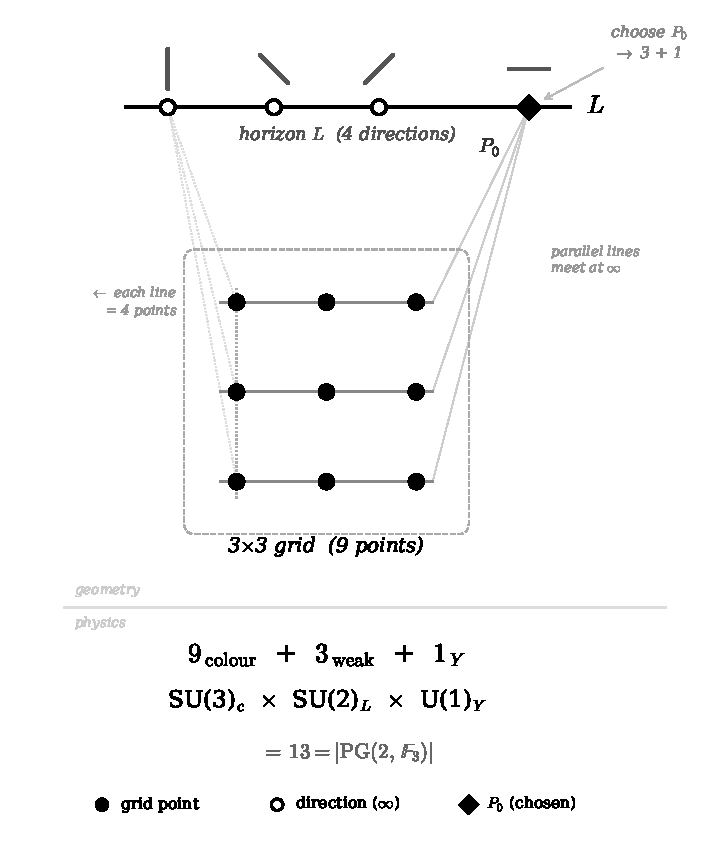
\includegraphics[width=0.75\columnwidth]{fig_pg23_v2.pdf}
\caption{The projective plane $\mathrm{PG}(2,\mathbb{F}_3)$.
Parallel lines on the $3 \times 3$ grid (9~points, filled circles)
meet at directions on the line at infinity~$L$ (open circles).
Choosing~$P_0$ (filled diamond) produces the partition
$9{+}3{+}1 = 13$, corresponding to the sector structure of
$\mathrm{SU}(3){\times}\mathrm{SU}(2){\times}\mathrm{U}(1)$.}
\label{fig:pg23}
\end{figure}

Under the full symmetry $\mathrm{PGL}(3, \mathbb{F}_3)$ of $\mathrm{PG}(2, \mathbb{F}_3)$, all 13 points are equivalent and no partition arises. We now fix one of the 4 points on the line at infinity~$L$ as a reference point~$P_0$---the pair $(P_0, L)$ is called a flag. Fixing the flag is a choice of reference within the construction: $\mathrm{PGL}(3, \mathbb{F}_3)$ acts transitively on flags, so every choice yields an isomorphic partition. The fixing splits the 13~points into three groups: 9 points off~$L$ (the $3\times 3$ grid),
3 points on~$L$ excluding~$P_0$, and~$P_0$ itself.
Choosing $P_0$ alone gives only $1{+}12 = {}$two groups;
choosing a flag produces $9{+}3{+}1$.
This is the minimal structure distinguishing three forces:
\begin{equation}
  \underbrace{N^2}_{9\;\mathrm{colour}} +
  \underbrace{N}_{3\;\mathrm{weak}} +
  \underbrace{1}_{1\;\mathrm{hyp}} = N^2 + N + 1.
\end{equation}

$N = d$ is satisfied only by $N = 3$ ($N = 2, 4, 5$ all have $d = 3 \neq N$). The primality of $N = 3$ guarantees that the field with $N$ elements is uniquely the prime field $\mathbb{F}_3 = \mathbb{Z}/3\mathbb{Z}$.
All numbers in the partition $9{+}3{+}1$ are determined by $N$ alone:
$N^2 = 9$, $N{+}1 = 4$ (excluding the reference point gives $N = 3$), reference point $1$.
Total: $N^2{+}N{+}1 = 13$.
The 52 flags (point-line incidence pairs) provide the basis for the Laplacian (\S\ref{sec:alpha}).

\subsection{From 13 Points to the Standard Model Gauge Group}

The partition $9{+}3{+}1$ matches the sector structure of the
Standard Model gauge group
$\mathrm{SU}(3){\times}\mathrm{SU}(2){\times}\mathrm{U}(1)_Y$.

\noindent\textbf{9~points $\to$ SU(3).}\;
The 9~off-line points constitute the affine plane
$\mathrm{AG}(2, \mathbb{F}_3)$.
These 9~points are labelled by $(a,b) \in \mathbb{F}_3^2$ and
naturally index the finite Weyl operators
$W_{\{a,b\}} = X^a Z^b$ in the three-dimensional internal
representation.
The identity $W_{\{0,0\}}$ is the central component; the remaining
8~non-trivial Weyl components form the traceless sector.
By the Killing--Cartan classification, the unique rank-2,
dimension-8 compact simple Lie completion is $\mathfrak{su}(3)$.
The 9th, central component corresponds to the global baryon number
$\mathrm{U}(1)_B$ (an ungauged global charge; the exact anomaly-free combination is $B{-}L$, \S8.4).

\noindent\textbf{3~points $\to$ SU(2).}\;
The 3~points on~$L$ excluding~$P_0$ give three non-trivial
weak directions relative to the reference point.
The minimal non-abelian compact Lie completion of these three
directions is the 3-generator $\mathfrak{su}(2)$, whose doublet
representation gives the weak $\mathrm{SU}(2)$ action.

\noindent\textbf{1~point $\to$ U(1)$_Y$.}\;
The reference point $P_0$ corresponds to the abelian central module phase, and physically to $\mathrm{U}(1)_Y$.

\noindent\textbf{Direct product guarantee.}\;
Translations of the affine plane fix the line at infinity~$L$---shifting the grid does not change the ``directions.''
The colour sector (9~points) transformations do not mix with the electroweak sector ($3{+}1$ points).
This is a geometric property following from the incidence structure of $\mathrm{PG}(2, \mathbb{F}_3)$: it yields a direct-product structure of three mutually non-mixing sectors---the same shape as the Standard-Model gauge group. The global form of the group (in the Standard Model, including the $\mathbb{Z}_6$ quotient~\cite{baezhuerta}) is not fixed by the geometry alone; it is determined by the faithful action on the particle carrier (Paper~II).

The complete derivation chain is:
{\small
\begin{equation}
\begin{gathered}
n^2{=}n
\;\xrightarrow{\;V=-H\;}
N{=}3
\;\xrightarrow{\;d=3\;}
\mathbb{F}_3^3
\;\xrightarrow{\;\text{count directions}\;}
13\text{ pts}\\
\;\xrightarrow{\;\text{flag}\;}
9{+}3{+}1
\;\xrightarrow{\;\text{Killing--Cartan}\;}
\mathfrak{su}(3){\oplus}\mathfrak{su}(2){\oplus}\mathfrak{u}(1).
\end{gathered}
\end{equation}
}
This mathematical result agrees with the experimentally
established gauge structure
$\mathrm{SU}(3) \times \mathrm{SU}(2) \times \mathrm{U}(1)$.

The 4~on-line points correspond to the four real degrees of freedom
of the $\mathrm{SU}(2)$ doublet --- the three Goldstone bosons
required for $\mathrm{SU}(2){\times}\mathrm{U}(1) \to
\mathrm{U}(1)_\mathrm{em}$ breaking and the physical Higgs.
$V = -H$ takes its minimum $-\ln 2$ at $\phi = 0$ ($\sigma = 1/2$)
and returns to zero as $\phi \to \pm\infty$.
This shape defines a stable well ($V''(0) = 1/4 > 0$). The vacuum sits at the interior point $\sigma = 1/2$ rather than at the vanishing-field points $\sigma \in \{0,1\}$---the role played in the Standard Model by the negative quadratic term ($\mu^2 > 0$), moving the vacuum from the symmetric point to a finite field value, is here played by the shape of the well.

\medskip
\noindent\textbf{Configuration decomposition of the existence variable $n$.}\;
The gauge structure creates diverse configurations within the
internal space of the existence variable $n$ (\S2). The variable
$n$ is unique --- by A3 (indiscernible $\Rightarrow$ identical),
bare existence with no distinguishing properties collapses to one. But the $\mathrm{PG}(2,\mathbb{F}_3)$
gauge structure defines multiple internal configurations: each
configuration $i$ is characterised by its generation
(bound state of $V = -H$) and gauge quantum numbers
(position in PG), and carries an occupation number
$n_i \in \{0,1\}$. $n$ is one, $n_i$ are many --- a unique
existence manifests as diverse fermions. The configuration
decomposition is:
\begin{equation}
  \sum_i \hat{n}_i = \hat{n}, \qquad
  \hat{n}_i^2 = \hat{n}_i, \qquad
  \hat{n}_i\,\hat{n}_j = \delta_{ij}\,\hat{n}_i.
\end{equation}
The first equation states that existence decomposes into
configurations; the second that bivalence ($n^2{=}n$) is
inherited by each configuration; the third that the unique unit of existence occupies exactly one configuration---the orthogonal resolution of the one-particle state space (the $\hat n_i$ are mutually orthogonal projections summing to $\hat n$). This mutual exclusivity is not an independent assumption but a consequence of the bivalence of existence~(A1) and its uniqueness~(A3). This is one-particle-level structure: the Pauli exclusion principle itself---no double occupancy of a single mode, together with exchange antisymmetry---is carried by the many-body realisation (the CAR construction)\PII{}, where distinct configurations can be simultaneously occupied. The concrete configuration labels are fixed by the fermion representations in \S5.3.
$n_i = 0$ does not mean non-existence; it
means existence occupies a different configuration.

\subsection{Origin of Fermion Diversity}

\S5.2 established that the 13 directions of $\mathrm{PG}(2,\mathbb{F}_3)$
give a structure with the same shape as the Standard-Model gauge group.
But the 13~directions do not correspond to fermions themselves.
The 13~directions define the gauge symmetry --- the structure of forces ---
and the fermion structure emerges as \textbf{representations} of this
gauge group.
Here we show why the single existence variable~$n$ gives rise to a
diverse matter-particle structure.

Before the gauge structure emerges, $n$ has no quantum numbers ---
no generation label, no colour, no isospin. Without distinguishing
properties, multiple instances of $n$ are identical
(Leibniz's principle of the identity of indiscernibles),
and $n$ remains unique.
The gauge structure of $\mathrm{PG}(2,\mathbb{F}_3)$ changes this:
the representations of the gauge group create diverse ``slots'' --- configurations ---
in the internal space, with each configuration carrying an occupation number $n_i \in \{0,1\}$.

Each configuration $i$ is characterised by two labels:
generation~$k$ (which bound state of $V = -H$, $k=1,2,3$) and gauge representation~$\alpha$
(which sector of $\mathrm{PG}(2, \mathbb{F}_3)$).
That is, $n_i = n_{k,\alpha}$.
The representations of $\mathrm{SU}(3){\times}\mathrm{SU}(2){\times}\mathrm{U}(1)$ give 16 states per generation. The chiral asymmetry ($\mathrm{SU}(2)$ acting only on left-handed fields) is part of this particle-species specification and is not derived in this paper. In Paper~II, under the stated enumeration conditions, mixed configurations are excluded and the left/right assignment is unique up to a global orientation convention.
The hypercharge values in the table below are the unique anomaly-free assignments compatible with the $9{+}3{+}1$ sector structure, Yukawa closure, the inclusion of~$\nu_R$, and the specification of a single local abelian gauge factor ($B{-}L$ remains an ungauged global charge, \S5.2); the operator-level derivation is likewise given in the same paper:

\vspace*{0.4\baselineskip}
\begin{center}
\small
\renewcommand{\arraystretch}{1.15}
\begin{tabular}{@{}l@{\qquad}l@{\qquad}l@{}}
\toprule
Representation & Content & States \\
\midrule
$(\mathbf{3},\mathbf{2},1/6)$ & Left-handed quarks $Q_L$ & 6 \\
$(\mathbf{3},\mathbf{1},2/3)$ & Right-handed up-type $u_R$ & 3 \\
$(\mathbf{3},\mathbf{1},-1/3)$ & Right-handed down-type $d_R$ & 3 \\
$(\mathbf{1},\mathbf{2},-1/2)$ & Left-handed leptons $L_L$ & 2 \\
$(\mathbf{1},\mathbf{1},-1)$ & Right-handed charged lepton $e_R$ & 1 \\
$(\mathbf{1},\mathbf{1},0)$ & Right-handed neutrino $\nu_R$ & 1 \\
\bottomrule
\end{tabular}
\end{center}
\noindent
Total: $16 \times 3$ generations $= 48$ configurations.
The inclusion of~$\nu_R$ is required for Yukawa closure
and for the $B{-}L$-protected Dirac-neutrino structure (see \S8.4 of this paper).
This is the concrete realisation of the configuration decomposition
above: the index $i$ runs over the pair $(k,\alpha)$, where $k$ is
the generation label and $\alpha$ is the gauge-representation label.
The inherited bivalence $n_i^2 = n_i$ is what, in the many-body realisation, restricts the occupation of each mode to $\{0,1\}$---this is the occupation-number representation of the Pauli exclusion principle~\cite{pauli}. The mutual exclusivity of distinct configurations is the one-particle-level structure of \S5.2: which configuration the unique unit of existence occupies. The generators of $\mathrm{SU}(3){\times}\mathrm{SU}(2){\times}\mathrm{U}(1)$
correspond to $8{+}3{+}1 = 12$ gauge bosons
(8~gluons, 3~weak bosons $W^+W^-Z$, 1~photon).
Together with the Higgs boson from~\S5.2, the 48~fermions, 12~gauge bosons,
and 1~Higgs constitute the complete particle content of the Standard Model.

Thus, diverse matter ($n_i$) arises from unique existence ($n$).
The key is that the gauge structure of $\mathrm{PG}(2, \mathbb{F}_3)$
creates ``distinguishable slots'' --- without gauge symmetry, existence
remains featureless and singular; with gauge symmetry, 48~species of
fermions emerge. The diversity of matter is a consequence of gauge structure.

The internal consistency of this construction is independently confirmed by the eigenfunction participation ratio $D_{PR} = (\int\rho\,d\phi)^2/\int\rho^2\,d\phi$, with $\rho = \sum_n \psi_n^2$ the total density of the three bound states, $= 13.06 \approx |\mathrm{PG}|$
(reproduced by the verification code) and by the spectral decomposition of the $52 \times 52$ flag Laplacian.\footnote{The finite-kernel theorem and its spectral gauge-decomposition corollary in Paper~II.}
No step in the derivation contains a free parameter.
The validity of this construction is supported by the fact that
all independent physical quantities derived in \S\ref{sec:couplings}--\ref{sec:results}
agree with experiment to $0.0006\%$--$2.6\%$ accuracy.

\section{Gauge Coupling Constants}\label{sec:couplings}
%=====================================================================

\S5.2 derived the structure corresponding to the gauge group
(which forces exist). This chapter derives their strengths
(coupling constants).

\subsection{Weinberg Angle}\label{sec:weinberg}

The partition $9{+}3{+}1$ of \S5.2 gives values corresponding
to the coupling constants.
The fraction of the 13~directions occupied by the 3~weak-sector
directions is the Weinberg angle~\cite{weinberg}
(weak mixing angle) $\sin^2\!\theta_W$.
The weight of each point is fixed by the symmetry prior to choosing
a flag: $\mathrm{PGL}(3,\mathbb{F}_3)$ acts transitively on
$\mathrm{PG}(2,3)$, so the 13~directions carry equal weight
(invariant measure). Fixing the flag does not alter these weights;
it only classifies the 13~points into $9{+}3{+}1$.
The Weinberg angle is read as the fraction that the 3 weak
directions occupy among all 13---taking all internal directions as the
denominator is one of the specified choices:
\begin{equation}\label{eq:weinberg}
  \sin^2\!\theta_W = \frac{N}{N^2{+}N{+}1} = \frac{3}{13} = 0.2308
  \qquad (\text{expt: } 0.23122\;\overline{\mathrm{MS}}\text{ at }M_Z,\; 0.2\%).
\end{equation}
The tree-level prediction $3/13 = 0.23077$
deviates from the $\overline{\mathrm{MS}}$-scheme experimental value
$0.23122 \pm 0.00003$~\cite{pdg} by $0.2\%$, consistent with one-loop radiative corrections.
This gives the tree-level $W/Z$ mass ratio:
$m_W/m_Z = \cos\theta_W = \sqrt{10/13} = 0.8771$ (expt: $0.8813$, $0.5\%$;
deviation consistent with radiative corrections).

\subsection{Strong Coupling Constant}\label{sec:strong}

The strong coupling constant follows by distributing the weak-sector
fraction over the rank of the colour sector.
Of the 9~colour-sector directions, the independent directions
number $\mathrm{rank}(\mathrm{SU}(3)) = 2$ (Cartan generators);
taking the readout that equidistributes $\sin^2\!\theta_W$ over
these 2 directions:
$\alpha_s^{(0)} = \sin^2\!\theta_W/(N{-}1) = 3/26 = 0.1154$ (this distribution rule is one of the specified choices).
The spectral marginality $\varepsilon = 0.219$ from \S\ref{sec:theorem}
provides the NLO correction.
The correction is distributed over $N^2{+}1 = 10$ non-weak
PG directions (colour~9 + hypercharge~1):
\begin{equation}\label{eq:alphas}
  \alpha_s = \frac{3}{26}\Bigl(1 + \frac{\varepsilon}{N^2{+}1}\Bigr) = 0.1179
  \qquad (\text{expt: } 0.1179\;\overline{\mathrm{MS}}\text{ at }M_Z,\; 0.01\%).
\end{equation}
The value $k = N^2{+}1 = 10$ follows from the number of non-weak directions in $\mathrm{PG}(2, \mathbb{F}_3)$. Throughout this paper the NLO corrections take the form
$1 \pm \ell\varepsilon/k$, where the denominator $k$ is the size of the
finite support over which the correction is distributed---$k = N^2{+}1 = 10$
for the non-weak sector ($\alpha_s$; affine $+$ hypercharge),
$k = N^2 = 9$ for generation mixing ($\sin\theta_C$; affine plane),
$k = |\mathrm{PG}| = 13$ for the full set of PG modes ($m_H/v$,
$\sin^2\!\theta_{23}$; full projective space), and $k = N = 3$ for the
three weak directions ($\sin^2\!\theta_{13}$). The assignment of
$(\ell, k)$ to each observable, including the sign and coefficient
$\ell$, is one of the specified choices.

\subsection{Fine-Structure Constant}\label{sec:alpha}

The Weinberg angle and strong coupling constant were determined
by simple point ratios on $\mathrm{PG}(2,3)$.
The fine-structure constant requires more---the full spectral
structure of the internal space.

The inverse electromagnetic coupling $1/\alpha$ measures the weakness of the electromagnetic interaction. The observed charge is the charge screened by the matter fields---the stronger the screening, the weaker the coupling and the larger $1/\alpha$. In this framework $1/\alpha$ is given (up to the self-consistent correction $-\alpha$) by the sum of the bare photon propagation cost $\lambda_1$ and the matter screening quantity $Z$, and the Thomson-point value is dominated by the screening term.
In 4D QED this structure is formalised as the Dyson equation.
In 0D the same structure holds but becomes algebraically
exact---the propagator is a constant, so the vertex correction
and self-energy are determined by the same resolvent, and the
4D perturbative cancellation $Z_1 = Z_2$ holds as an exact
algebraic identity (proof in Paper~II).
The self-consistency equation is:
\begin{equation}\label{eq:alpha_sc}
  \frac{1}{\alpha} + \alpha = \lambda_1 + Z.
\end{equation}
The right-hand side has two terms:
$\lambda_1$ is the bare photon inverse propagator
(propagation cost) and $Z$ corresponds to the scalar-channel spectral quantity (screening). This correspondence is a spectral one---$Z$ is the resolvent trace
whose energy-denominator structure matches the matter vacuum polarisation. The form of the equation (the left-hand side $1/\alpha + \alpha$ with unit coefficient) belongs to the specified correspondence of the incidence current with the Thomson-point electromagnetic current. The full justification of this correspondence as a self-consistent prediction, and the proof that the physical root is unique under this reading, are both given in the same paper. The dominant contribution to $Z$ is $1/|E_2| = 95.94$; since $E_2$ is rigorously certified by the interval arithmetic of \S\ref{sec:rigorous}, this sensitivity introduces no uncertainty.

The minimum cost $\lambda_1$ for gauge-field propagation through
internal space is the smallest non-zero eigenvalue of the Laplacian
on internal space.
Since gauge interactions involve both positions (points) and
directions (lines), the natural object for diffusion is a
flag (point-line incidence pair).
The spectrum of the graph Laplacian $\mathcal{L}$ on the flag graph of
$\mathrm{PG}(2,\mathbb{F}_3)$, a $52 \times 52$ matrix, is:
\begin{center}\small
\begin{tabular}{ccl}
\toprule
Eigenvalue & Value at $N=3$ & Multiplicity \\
\midrule
$0$ & $0$ & $1$ \\
$(N{+}1) - \sqrt{N}$ & $2.268$ & $12$ \\
$(N{+}1) + \sqrt{N}$ & $5.732$ & $12$ \\
$2(N{+}1)$ & $8$ & $27$ \\
\bottomrule
\end{tabular}
\end{center}
\noindent
The smallest non-zero eigenvalue $\lambda_1 = 4 - \sqrt{3} = 2.268$ is the quantity that corresponds to the bare photon inverse propagator in the $1/\alpha$ correspondence (\S6.3). $\lambda_1 > 0$ is consistent with the confinement picture---the positive spectral gap corresponds to colour-charged states not propagating freely in the asymptotic regime.

The screening term $Z$ corresponds to the scalar-channel spectral quantity from three generations of matter fields,
determined by the resolvent of the internal kinetic operator.
The internal kinetic operator is a tensor sum of the
generation sector ($K_\mathrm{gen}$, whose eigenvalues are the binding
energies $|E_n|$) and the gauge sector ($\mathcal{L}$, eigenvalues $\lambda_k$):
\[
  K_\mathrm{int} = K_\mathrm{gen} \otimes \mathbf{1}
    + \mathbf{1} \otimes \mathcal{L}
\]
This form---the tensor sum, with both factors measured in the same unit at relative scale 1---is established as a uniqueness theorem\PII{} under the single-clock unit clause (product couplings, twisted products, and rescalings of the relative unit are excluded). Decomposing the trace of the resolvent by multiplicity:
\[
  Z = \mathrm{Tr}[1/K_\mathrm{int}]
    = \zeta_V(1) + 12\,S_1 + 12\,S_2 + 27\,S_3 = 134.77613
\]
where $\zeta_V(1) = \sum_n |E_n|^{-1}$ and
$S_i = \sum_n (|E_n| + \lambda_i)^{-1}$.
The intermediate values are:
$\zeta_V(1) = 104.28714$ (dominated by $E_2^{-1} = 95.94$), $12S_1 = 14.57025$, $12S_2 = 6.05684$, $27S_3 = 9.86190$.
The 27-dimensional sector (multiplicity $27 = 3^3$) contributes
$9.86 \approx N^2$, providing the spectral structure corresponding to the QCD vacuum-polarisation correction
(all intermediate values are reproducible with the
accompanying verification code).

Substituting $\lambda_1 = 4-\sqrt3 = 2.26795$ and $Z = 134.77613$ into the self-consistency equation:\footnote{The recommended experimental value is $1/\alpha = 137.035999177(21)$ (CODATA 2022). The value 137.0368 in the text is the leading term; the high-precision evaluation including the correction series is treated in Paper~II.}
\begin{equation}\label{eq:137}
  \frac{1}{\alpha} = \frac{(Z{+}\lambda_1)
    + \sqrt{(Z{+}\lambda_1)^2 - 4}}{2} = 137.0368
  \quad(\text{expt: } 137.036,\; 0.0006\%).
\end{equation}

\section{Higgs Sector and Electroweak Symmetry Breaking}\label{sec:higgs}

\S6 derived the gauge coupling constants. The Standard Model has one more
free parameter in the scalar sector --- the Higgs self-coupling~$\lambda$.
This chapter derives the mathematical structure corresponding to it and shows the pinning of the internal vacuum and the boundedness of the internal potential (no instability channel).

\subsection{Symmetry Breaking and Higgs Mass}\label{sec:higgs-mass}

Electroweak symmetry breaking is the statement that, while the dynamical laws remain symmetric, the vacuum (ground state) departs from the symmetric point. Since the $W$ and $Z$ are massive while the photon is massless, the vacuum cannot sit at the field-vanishing point (the symmetric point)---breaking is required by experiment. The Standard Model realises this through the assumption $\mu^2 > 0$ in the Higgs potential $V = -\mu^2|\Phi|^2 + \lambda|\Phi|^4$: it destabilises the origin, rolling the field to a finite value. But ``why $\mu^2 > 0$'' is not explained within the Standard Model.

The $V = -H(\sigma(\phi))$ of this paper answers this question through structure. The binary Shannon entropy $H$ vanishes at both endpoints $\sigma \in \{0,1\}$ (the trivial configurations corresponding to the field-vanishing point) and is maximal at the interior point $\sigma = 1/2$, so $V = -H$ is a stable well that is 0 at the endpoints and reaches its minimum $-\ln 2$ at the interior point ($V''(0) = 1/4 > 0$). Moreover A2 ($\sigma \neq 1$) and A3 ($\sigma \neq 0$) forbid the endpoints themselves. The ground state therefore necessarily sits at the interior point---the condition that the vacuum cannot sit at the symmetric point, i.e.\ the condition for breaking, follows from the shape of the entropy and the axioms rather than from destabilising the origin. The position of the vacuum is a consequence of the shape of $V$ and requires no additional assumption. The readout of the Higgs mass uses the positive curvature $V''(0) = 1/4$ at this minimum.

\S5.2 showed that the line structure of $\mathrm{PG}(2,\mathbb{F}_3)$
corresponds to the Higgs $\mathrm{SU}(2)$ doublet. The curvature at the
centre gives the Higgs mass:
$V''(0) = g_F(0) = \sigma(0)(1{-}\sigma(0)) = 1/4$
(the Fisher metric at $\sigma = 1/2$).
\begin{equation}
  m_H/v = \sqrt{V''(0)} = 1/2 \quad (\mathrm{LO}).
\end{equation}
The NLO correction enters from all $|\mathrm{PG}| = 13$ modes of the Laplacian matrix $\mathcal{L}$:
\begin{equation}\label{eq:higgs}
  m_H/v = \frac{1}{2}\sqrt{1 + 2\varepsilon/|\mathrm{PG}|}
  = 0.5084 \quad (\text{experiment: } 0.5082,\; 0.03\%).
\end{equation}
This corresponds to $\lambda = (m_H/v)^2/2 = 0.1292$ (expt: 0.1291, 0.06\%).

\subsection{Vacuum Stability and the Hierarchy Problem}

The Standard Model Higgs potential $V_\mathrm{SM} = -\mu^2 h^2 + \lambda h^4$ diverges
as $h \to \infty$, and the UV correction $\delta\mu^2 \propto \Lambda^2$
requires $\sim 10^{34}$ fine-tuning between the electroweak and Planck scales (hierarchy problem).
Furthermore, the Higgs quartic coupling $\lambda(\mu)$ runs negative at $\mu \sim 10^{10}$\,GeV, making the electroweak vacuum cosmologically metastable.

In the internal sector of $V = -H$, the instabilities corresponding to
these problems do not arise.
$V = -H$ is bounded ($|V| \leq \ln 2$), with no high-energy divergence.
The well depth $|V_{\min}| = \ln 2$ and curvature $V''(0) = 1/4$
are both $O(1)$ algebraic constants;
their ratio gives
$|V_{\min}|/V''(0) = 4\ln 2 \approx 2.77$, a ratio of internal quantities,
an order-unity number requiring no fine-tuning (its correspondence to the 4D $v^2/\Lambda^2$ requires the reconstruction matching).
The internal potential $V = -H$ is bounded: $V \in [-\ln 2, 0]$. Interpreting this boundedness as the reason the running coupling $\lambda(\mu)$ in 4D does not turn negative requires the reconstruction matching (likewise the full 4D vacuum-stability interpretation and the correspondence to thermal properties such as symmetry restoration at high temperature)\PII{}.
The shape of $V$ is fixed by the axioms, and scale dependence does not alter the algebraic structure of $V$.
Furthermore, $V = -H$ is uniquely determined as the
canonical free energy of $n \in \{0,1\}$ (\S2).
Within the minimal PFE operator algebra, no second fundamental
scalar potential is generated.
The minimal reconstruction thus predicts a single Higgs doublet.

\subsection{Radiative Corrections and Summary of Couplings}

\noindent\textbf{Radiative corrections.}\;
The predictions above are algebraic values, and their comparison with $M_Z$-scale experiments requires the 4D RG evolution and loop corrections of the running quantities (\S\ref{sec:correspondence}).
The next correction to the weak angle is fixed in closed form by the framework's own readout: $\Delta_\mathrm{rad} = \alpha\cdot 5N^3\!/|\mathrm{PG}|^3 = \alpha\cdot 135/2197 = 0.00045$ (derived in the same paper under the specified readout). This gives $\sin^2\!\theta_W = 3/13 + \Delta_\mathrm{rad} = 0.23077 + 0.00045 = 0.23122$, in agreement with the $\overline{\mathrm{MS}}$ value $0.23122 \pm 0.00003$~\cite{pdg} within errors. Similarly, the leading value $m_W/m_Z = \sqrt{10/13} = 0.8771$ is $0.5\%$ below experiment; this residual has approximately the size and sign of the standard SM top-quark $\Delta\rho$ correction, but the $\Delta\rho$-corrected comparison is a conditional computation requiring renormalisation-scheme matching.

\noindent\textbf{Summary.}\;
$\sin^2\!\theta_W(M_Z) = 0.23122$ ($<0.01\%$),
$\alpha_s(M_Z) = 0.1179$ (0.01\%),
$1/\alpha_\mathrm{em} = 137.0368$ (0.0006\%),
$m_H/v = 0.5084$ (0.03\%).
All four coupling constants are derived from $V = -H$ and $\mathrm{PG}(2,3)$ and agree with experiment. The vacuum is pinned at an interior point, the internal potential is bounded (no instability channel), and there is only one Higgs. The correspondence to 4D vacuum stability and the hierarchy problem is a matter of reconstruction matching.


\section{Fermion Masses and Mixing}\label{sec:physics}
%=====================================================================

\S5--7 established the structures corresponding to gauge structure,
coupling constants, and the Higgs mass.
Based on the correspondence between the three bound states established in \S\ref{sec:theorem}
and the three generations of charged leptons, this chapter derives
formulas for the mass ratios and mixing angles from the localisation
of the bound states.
The derived values agree to high precision with the mass ratios
of charged leptons, quarks, and neutrinos,
and with the CKM/PMNS mixing angles.

%=====================================================================
\subsection{Mass Formula}\label{sec:mass}

The three bound states of $V = -H$ differ in localisation.
The deepest $\psi_0$ is localised at the well bottom and couples
most strongly to the gauge field, corresponding to the heaviest $\tau$:
\begin{center}\small
\begin{tabular}{lcccc}
\toprule
Bound state & Energy & Localisation & Particle & Mass (MeV) \\
\midrule
$\psi_0$ & $E_0 = -0.485$ & High (well bottom) & $\tau$ & 1777 \\
$\psi_1$ & $E_1 = -0.159$ & Medium & $\mu$ & 106 \\
$\psi_2$ & $E_2 = -0.010$ & Low (well edge) & $e$ & 0.511 \\
\bottomrule
\end{tabular}
\end{center}

\noindent
The mass ratios are determined by the localisation of the wave
functions, not as independent parameters.
The key quantity is $R = \ln(m_\tau/m_e)/\ln(m_\mu/m_e)$,
which compresses the three-body mass hierarchy into a single
number.
\begin{equation}
  V = -H \;\xrightarrow{\;\text{\S3}\;} \psi_n
  \;\xrightarrow{\;\text{IPR}\;} \mathrm{localisation}
  \;\xrightarrow{\;2C_F\;} m_n
  \;\xrightarrow{\;} R = 1.5293
\end{equation}

Each eigenstate has a binding energy $|E_n|$ and a localisation.
Localisation is measured by the inverse participation ratio
$\mathrm{IPR}_n = \int|\psi_n|^4\,d\phi$.
The coupling strength to the gauge field is proportional to the
wave-function amplitude at the interaction point.
A more localised state in internal space has a larger amplitude at
that point and acquires a larger mass via the gauge field.
Mass is proportional to a power of localisation:
$m_n \propto \mathrm{IPR}_n^b$.
In this section's readout, the exponent $b$ is taken to be the internal-localisation Casimir of the continuous $\mathrm{SU}(3)$ lift associated with the $N = 3$ sector: $b = 2C_F = (N^2{-}1)/N = 8/3$.\footnote{This is not the physical colour charge of leptons but the $N = 3$ internal-localisation Casimir; for quarks the same $N = 3$ structure coincides with colour. See Paper~II~\cite{paper2}.}

A small correction arises from the anharmonicity of $V = -H$.
Each mode samples the well differently;
the virial ratio $|\langle V \rangle_n| / T_n$
(ratio of potential to kinetic energy) measures this.
The correction exponent is determined by the spectral
$\zeta$-function through the marginality parameter: the semiclassical
action count $n_\mathrm{WKB} = 2.781$ falls short of the exact
bound-state count $N = 3$ by $\varepsilon = 0.219$,
giving a per-mode marginality $\delta = \varepsilon/N = 0.073$.

The complete mass formula is:
\begin{equation}\label{eq:mass}
  m_n \propto |E_n| \times \mathrm{IPR}_n^{2C_F}
  \times \Bigl(\frac{|\langle V \rangle_n|}{T_n}\Bigr)^{\varepsilon/N}.
\end{equation}
The three factors have different origins:

\begin{center}\small
\begin{tabular}{lll}
\toprule
Factor & Physical meaning & Determined by \\
\midrule
$|E_n|$ & Energy scale & Binding energy \\
$\mathrm{IPR}^{2C_F}$ & Localisation $\to$ coupling strength & Group theory (Casimir) \\
$(|\langle V \rangle|/T)^{\varepsilon/N}$ & Anharmonic correction & Spectral marginality \\
\bottomrule
\end{tabular}
\end{center}

\noindent
All exponents are determined by $V = -H$.
The result:\footnote{All spectral quantities are computed with
$|\phi|_\mathrm{max} = 100$, $\Delta\phi = 1.25\times 10^{-4}$
($N_\mathrm{grid} = 1600001$), verified stable under
doubling of grid resolution and box enlargement.}
\begin{equation}
  R = \frac{\ln(m_\tau/m_e)}{\ln(m_\mu/m_e)} = 1.5293
  \qquad (\text{experiment: } 1.5294,\; 0.006\%).
\end{equation}
The readout of this section fixes the group-theoretic Casimir $b = 2C_F = 8/3$ first.
Substituting this fixed value, both the Koide~\cite{koide} constraint
$Q \approx 3/2$ (our convention is $Q = (\sum\sqrt{m})^2/\sum m$, the inverse of the standard convention $\sum m/(\sum\sqrt{m})^2 = 2/3$) and the spectral condition $c = \varepsilon/N$
are independently satisfied.
Koide is therefore not an input that determines~$b$, but an
output check of $b = 8/3$:
  \begin{center}\small
  \begin{tabular}{ccc}
  \toprule
  $b$ & $c\,(Q{=}3/2)$ & Deviation \\
  \midrule
  $2.0$ & $0.437$ & $500\%$ \\
  $2.5$ & $0.163$ & $120\%$ \\
  $\mathbf{8/3 = 2C_F}$ & $\mathbf{0.0730}$ & $\mathbf{0.07\%}$ \\
  $2.78$ & $0.012$ & $84\%$ \\
  $3.0$ & $-0.107$ & $246\%$ \\
  \bottomrule
  \end{tabular}
  \end{center}

\noindent
The individual mass ratios:
\begin{center}\small
\begin{tabular}{lccc}
\toprule
 & Prediction & Experiment & Accuracy \\
\midrule
$m_\tau/m_e$ & 3481 & 3477 & 0.1\% \\
$m_\mu/m_e$ & 207.0 & 206.8 & 0.1\% \\
$R$          & 1.5293 & 1.5294 & 0.006\% \\
$Q$ (Koide)  & 1.499985 & 1.50001(2) & $2\sigma$ (from PDG masses) \\
\bottomrule
\end{tabular}
\end{center}

The three lepton masses are not independent parameters but three modes of a single well, with the exponent $2C_F = 8/3$ fixed by this section's readout. In 0D there are no loop integrals, so nothing generates an anomalous dimension dynamically. The Peter--Weyl theorem for finite groups guarantees that the heat kernel on the group is a finite sum $K(t) = \sum_\rho \dim(\rho)\,\chi_\rho(g)\,e^{-\lambda_\rho t}$, admitting only exponential decay with no power-law terms. The exponent is therefore fixed by the representation, and taking its value to be the internal-localisation Casimir $2C_F$ of the continuous SU(3) lift is the readout of this section.\footnote{The uniqueness of this readout is treated in Paper II: the functional form of the mass response is proved as a uniqueness theorem, and the exponent assignment is treated as an explicitly specified readout.} The $0.006\%$ agreement of $R = 1.5293$ quantitatively supports the correspondence between bound states and lepton generations. The stability of the Koide relation under radiative corrections is discussed by Sumino~\cite{sumino}.


\subsection{Quark Masses}\label{sec:quarks}

The mass formula of \S\ref{sec:mass} reproduced $R = 1.5293$ for leptons.
Can the same formula be applied to quarks?
The formula itself does not change---only the well depth changes.

Leptons are colour singlets and feel $V = -H$ as a single copy.
Quarks carry three colours. The colour-triplet well is taken to be $V = -3H$, the sum of the three isomorphic colour contributions on the common existence coordinate $\phi$---another of the specified choices.
The deeper well supports 5~bound states ($n_\mathrm{WKB} = 4.82$). In the tables below,
$\kappa$ denotes the well-depth multiplier (the $\kappa$ in $V = -\kappa H$):

\begin{center}\small
\begin{tabular}{lcccc}
\toprule
Sector & Operator & $\kappa$ & Bound states & Modes used \\
\midrule
Lepton & $-H$  & 1 & 3 & $(0,1,2) = \tau,\mu,e$ \\
Up-type & $-3H$ & 3 & 5 & $(1,2,3) = t,c,u$ \\
Down-type & $-3H$ (corr.\ in kinetic term) & 3 & 4 & $(0,1,2) = b,s,d$ \\
\bottomrule
\end{tabular}
\end{center}

\noindent\textbf{Up-type.}\;
Mode~0 is deeply confined and belongs to the $I_3 = -1/2$ sector.
Up-type quarks ($I_3 = +1/2$) use modes $(1,2,3)$, giving
$R_\mathrm{up} = 1.777$ (experiment: $1.770$, $0.4\%$).

\noindent\textbf{Down-type.}\;
Up-type and down-type belong to the same $\mathrm{SU}(2)$
doublet and feel the same $V = -3H$, but differ in the sign of
weak isospin ($I_3 = +1/2$ vs $-1/2$).
This sign supplies a correction to the mass formula.

The total gauge charge of the $\mathrm{SU}(2)$ doublet $(u, d)$, $2C_F + 1/N_c = N_c$, is an exact algebraic identity.
The physical mechanism originates from
$\mathrm{PG}(2,\mathbb{F}_3)$ geometry: among the $N{+}1 = 4$ points on
line~$L$, the reference point~$P_0$ is the reference that orients the
doublet (which component is called $I_3 = +1/2$), and the
remaining 3~points generate $\mathrm{SU}(2)$. Reversing this
orientation flips the sign of $I_3$ and reverses the $\mathrm{SU}(2)$
action, coupling the total charge~$N_c$ to $g_F(\phi) = \sigma(1{-}\sigma)$
(the Bernoulli Fisher metric $g_F = \operatorname{Var}(n)$ of \S\ref{sec:partition}; its uniqueness is \v{C}encov's theorem~\cite{cencov}) with
a negative sign.
The effective mass is:
\begin{equation}
  m_\mathrm{eff}(\phi) = 1 - N_c\,\sigma(1{-}\sigma)
\end{equation}
This is the static Fisher-limit form of the down-sector readout. The operator actually solved is the symmetric position-dependent-mass form $-\tfrac{1}{2}\,\partial_\phi\,(1/m_\mathrm{eff})\,\partial_\phi - 3H$ (identical to the discretisation in the accompanying code).
The correction coefficient $g_c = -N_c = -3$ (distinct from the normalisation $g$ of \S2.4) is fixed by the algebraic structure of the $\mathrm{SU}(2)$ doublet. The corrected operator has 4 negative eigenvalues ($-1.5709$, $-0.5455$, $-0.1952$, $-0.00733$; stable for box size $L_\mathrm{box} = 40/80/120$), of which 3 modes $(0,1,2)$ correspond to the physical window $b, s, d$---which modes form the physical window is, as for the up-type sector, a readout specification (the window differs sector by sector: all 3~modes for leptons, $(1,2,3)$ for up-type, $(0,1,2)$ for down-type). With modes $(0,1,2)$: $R_\mathrm{down} = 2.273$ (experiment: $2.276$, $0.1\%$).

The mass ratios of all three charged-fermion sectors are reproduced:

\begin{center}\small
\begin{tabular}{lccccc}
\toprule
Sector & $\kappa$ & $g_c$ & $R$ (pred.) & $R$ (expt.) & Accuracy \\
\midrule
Lepton  & 1 & 0 & 1.529 & 1.529 & 0.006\% \\
Up      & $N_c = 3$ & 0 & 1.777 & 1.770 & 0.4\% \\
Down    & $N_c = 3$ & $-N_c$ & 2.273 & 2.276 & 0.1\% \\
\bottomrule
\end{tabular}
\end{center}

\noindent Here $R$ captures the shape of the log-hierarchy---it is invariant under a uniform stretching of the mass ratios (raising every $m_i/m_j$ to a common power)---not the individual masses. The accuracy column gives the deviation of the prediction from the experimental central value. The experimental $R$ inherits the light-quark mass uncertainties (PDG 2026: $m_u = 2.16 \pm 0.07$ MeV, etc.), which propagate to a width of about $\pm0.15$--$0.25\%$, and the comparison further depends on the scheme and scale conventions for each mass (light quarks $\overline{\mathrm{MS}}$ at 2 GeV, $c$ and $b$ at $m(m)$, $t$ from direct measurement). Which of the modes correspond to which quarks is a physical specification (which 3 of the 5 modes), not a derivation.\footnote{The individual quark magnitudes are treated conditionally in Paper~II.}

\subsection{CKM Mixing}\label{sec:ckm}

\S8.1--8.2 established the mass ratios. With masses determined,
we now derive the inter-generation mixing~\cite{km}.
Why is $V_{ub}$ small, and why does the Cabibbo angle~\cite{cabibbo}
take its particular value?
The Standard Model does not explain these.
In $V = -H$, the potential symmetry corresponds to the former
and the marginality of the third generation to the latter.

The potential $V = -H$ is symmetric: $V(\phi) = V(-\phi)$.
This fixes the parity of each eigenfunction: $\psi_0$ even, $\psi_1$ odd, $\psi_2$ even. The direct overlap between distinct modes vanishes by Sturm--Liouville orthogonality: $\langle\psi_0|\psi_2\rangle = 0$. Since $\psi_0$ and $\psi_2$ are both even, $\langle\psi_0|M|\psi_2\rangle = 0$ for a $V$-parity-odd mixing operator $M$---the leading $0\leftrightarrow 2$ transition is forbidden:
\begin{equation}
  V_{ub}\big|_\mathrm{tree} = 0
\end{equation}
The observed value $|V_{ub}| \approx 0.004$ arises at higher orders of the Wolfenstein hierarchy~\cite{wolfenstein}. V-parity makes the tree/direct term exactly zero and suppresses distant-generation transitions to at least $O(\varepsilon^3)$; in the Paper~II readout, the first non-zero term is $2\varepsilon^4$ (see below).

The Cabibbo angle follows from spectral marginality.
The third bound state $\psi_2$ is marginally bound---its binding
energy $|E_2| = 0.010$ is only $1.5\%$ of the well depth.
The parameter measuring this marginality is the gap between the exact
bound-state count and the semiclassical action count:
$\varepsilon = N - n_\mathrm{WKB} = 3 - 2.781 = 0.219$.

Mixing angles reflect the mismatch between mass and weak
eigenstates; the marginality of the third bound state
($\varepsilon > 0$) is the source of mixing, and
$\varepsilon \to 0$ removes it,
leaving the three generations intact but with vanishing flavour transitions.
The readout expressing the angle as a series in $\varepsilon$---which
operator carries the transition, and what fixes its order and
denominator---is part of the specified choices (see the list in \S6.2).
To second order:
\begin{equation}\label{eq:cabibbo}
  \sin\theta_C = \varepsilon\Bigl(1 + \frac{\varepsilon}{N^2}\Bigr) = 0.2245   \qquad (\text{experiment: } 0.2243,\; 0.10\%).
\end{equation}
This value is the unscreened internal value. The observed readout composed with colour screening is $\sin\theta_C \cdot (1-x) = 0.22435$ ($x = N^2\alpha/(2\pi|\mathrm{PG}|) = 9\alpha/(26\pi)$ is the colour-screening expansion parameter; derived in the same paper).

The Cabibbo angle is a direct expression of the fact that the third generation barely exists: the generation-sector spectral quantity $\varepsilon = 0.219$, defined in \S\ref{sec:theorem} from $V = -H$ alone and entering all mixing readouts in common. If the third bound state were slightly more deeply bound ($\varepsilon \to 0$), inter-generation mixing would vanish and all flavour transitions would be forbidden.

The Wolfenstein hierarchy follows from the Cabibbo angle~\cite{wolfenstein}: $|V_{us}| \sim \varepsilon$, $|V_{cb}| \sim \varepsilon^2$, and $|V_{ub}|$ is suppressed to at least $O(\varepsilon^3)$ with first non-zero term $2\varepsilon^4$ (experiment: $0.225$, $0.041$, $0.004$).
NLO corrections take the form $1 \pm \ell\varepsilon/k$. The assignment
of the denominator $k$ and of the sign and coefficient $\ell$ is as
listed in \S6.2 ($1+\varepsilon/9$ for $\sin\theta_C$,
$1-2\varepsilon/3$ for $\sin^2\!\theta_{13}$).

The parity symmetry $V(\phi) = V(-\phi)$ suppresses the direct
$0\leftrightarrow2$ flavour transition, but it does not by itself fix
the QCD vacuum angle: parity alone leaves $\theta\in\{0,\pi\}$.
The observable strong-CP angle is $\bar\theta = \theta_\mathrm{QCD} + \arg\det M_q$. The strong-CP matching theorem of Paper~II shows that applying A1--A3 so as to preserve not only the finite internal observables but also the generating action words, the regularised fermion determinant line and the realisation of large gauge loops gives both $\arg\det(M_uM_d) = 0$ and a vanishing bare $\theta_\mathrm{QCD}$, hence $\bar\theta(\mu_0) = 0$ at the matching point of the minimal PFE reconstruction. What kills the bare QCD angle there is the fact that the only unitary scalar preserving the positive measure ray is $\{1\}$ (the ordered-measure-line triviality lemma of Paper~II)---not $V$-parity on its own. This is a statement at the matching point and not an exact zero at all scales: $\bar\theta_\mathrm{IR}$, which includes weak CKM loops and thresholds, is left unevaluated in Paper~II as well. Consequently, beyond a PQ-type axion---excluded by the absence of a PQ-type global U(1)---no claim is made about the non-existence of axion-like particles in general. Yet CP violation \emph{is} observed in the CKM sector ($J = 3.08 \times 10^{-5}$). This is consistent with the bare $\theta_\mathrm{QCD} = 0$: the CKM phase arises at higher order in $\varepsilon$ ($J = \pi\varepsilon^5/N_\mathrm{flags}$ with $N_\mathrm{flags} = 52$ the total number of flags (\S5.1)---a theorem under the readout specified in the same paper), while the matching-point condition remains exactly zero.

The flavour and strong-CP results are summarised:
\medskip
\begin{center}\footnotesize
\begin{tabular}{@{}p{0.27\linewidth}p{0.32\linewidth}p{0.33\linewidth}@{}}
\toprule
Quantity & Prediction & Experiment \\
\midrule
$V_{ub}$ (tree) & 0 (first non-zero term $2\varepsilon^4$, Paper~II) & $|V_{ub}| = 0.004$ (generated at higher order) \\
Bare $\theta_\mathrm{QCD}$ & \textbf{Not a consequence of $V$-parity} (matching-point value $\bar\theta(\mu_0)=0$; the measure-line triviality lemma and strong-CP matching theorem of Paper~II) & $\bar\theta < 10^{-10}$ \\
CKM CP violation & $J = \pi\varepsilon^5/N_\mathrm{flags}$ (theorem under the Paper~II readout) & $3.06 \times 10^{-5}$ (expt $3.08{\times}10^{-5}$) \\
\bottomrule
\end{tabular}
\end{center}
\bigskip

\subsection{Neutrinos}\label{sec:neutrinos}

\S8.1--8.3 derived charged-fermion mass ratios and mixing angles.
What remains are the neutrinos.

\noindent\textbf{Mass predictions.}\;
Neutrinos are colour singlets with $\kappa = 1$, coupling to $V = -H$---the same potential as charged leptons. The mass ratio $R$ depends only on the well shape (IPR and virial ratios), not on particle species. The same well gives the same $R$: $R_\nu = R_\mathrm{lepton} = 1.529$---this is the input-free prediction of this section. Conditional on the normal-ordering branch and the measured oscillation splittings~\cite{nufit} ($\Delta m^2_{21} = 7.537 \times 10^{-5}\;\mathrm{eV}^2$, $\Delta m^2_{31} = 2.521 \times 10^{-3}\;\mathrm{eV}^2$), this ratio fixes the absolute masses\footnote{The $\pm 0.03\;\mathrm{meV}$ uncertainty propagates from oscillation data input; the theory has no free parameters. Normal ordering is an input condition in this section; its independent derivation is given as a theorem\PII{} (a consequence of $R_\nu > 1$ and $(m_3/m_2)^2 = 169/5 > 1$).}:

\begin{center}\small
\begin{tabular}{lll}
\toprule
Quantity & Prediction & Status \\
\midrule
$m_1$ & $0.32 \pm 0.03\;\mathrm{meV}$ & Unmeasured \\
$m_2$ & $8.69\;\mathrm{meV}$  & Consistent \\
$m_3$ & $50.2\;\mathrm{meV}$ & Consistent \\
$\sum m_i$ & $59.2 \pm 0.3\;\mathrm{meV}$ & Below Planck ($<120$) \\
\bottomrule
\end{tabular}
\end{center}

What the flag-Laplacian spectrum fixes exactly is $m_3/m_2 = |\mathrm{PG}|/\sqrt{N{+}2} = 13/\sqrt{5}$, i.e.\ $(m_3/m_2)^2 = 169/5$. The mass-squared-difference ratio is given by the master relation $\Delta m^2_{31}/\Delta m^2_{21} = (169/5 - t^2)/(1 - t^2) = 33.842\ldots$ (displayed as 33.84), obtained by eliminating $t = m_1/m_2$ using $R_\nu = R_\mathrm{lepton}$\PII{}. With non-zero $m_1$, $169/5$ is not the exact value of the mass-squared-difference ratio. The ratio of the $\Delta m^2$ inputs used in this section is itself $2.521/0.07537 = 33.45$, whereas the master relation gives $33.84$ without oscillation input. This $1.2\%$ is the difference between the theoretical value and the present measurement. Since the absolute masses in the table above are conditional on the input ratio, using the master-relation value instead raises $m_3$ and $\Sigma m_\nu$ by about $0.6\%$ (the table gives $m_3/m_2 = 5.777$ against $13/\sqrt5 = 5.814$).

This prediction is falsifiable: the conditional calculation of this section does not itself test the mass ordering, but $\sum m_i > 70\;\mathrm{meV}$ creates tension. Since $\Sigma m_i = 59.2\;\mathrm{meV}$ lies close to the general normal-ordering minimum ($58.89\;\mathrm{meV}$ at $m_1 \to 0$), a CMB-S4~\cite{cmbs4} ($\sigma \sim 15\;\mathrm{meV}$) detection near this value would confirm the normal ordering but not distinguish this framework from the general minimal scenario; the sharp, framework-specific neutrino prediction is the ratio $\Delta m^2_{31}/\Delta m^2_{21} = 33.8$, testable by JUNO in 2026--27.

\noindent\textbf{Mixing angles.}\;
In \S\ref{sec:ckm}, CKM mixing angles were obtained from
$\varepsilon = 0.219$---small values ($\sin\theta_C \approx 0.22$).
Yet PMNS mixing angles are large
($\sin^2\!\theta_{12} \approx 1/3$).
Why does the same $V = -H$ produce both small and large mixing?

The answer lies in colour charge. Quarks carry colour and reside in the deep well $V = -3H$, which places their mixing in the perturbative regime of small mode overlap---this is why quark mixing is small, and its expansion parameter is the generation-sector marginality $\varepsilon$ (\S\ref{sec:theorem}).
Neutrinos are colour-neutral; instead, the geometric allocation
of gauge directions on $\mathrm{PG}(2,3)$ directly gives values
corresponding to the mixing angles.
The solar angle is the fraction of one complete electroweak line
($N{+}1 = 4$ points) in the 13~directions of $\mathrm{PG}$:
\begin{equation}
  \sin^2\!\theta_{12} = \frac{N{+}1}{|\mathrm{PG}|}
  = \frac{4}{13} = 0.3077
  \qquad (\text{experiment: } 0.3088,\; 0.4\%).
\end{equation}
At LO the atmospheric angle is the fraction that the disjoint union of the $N$ pure-weak directions and another line through the reference point ($N{+}1$ points) occupies among the 13 directions of PG, namely $7/13$. With the PG-scale NLO correction ($k = |\mathrm{PG}| = 13$):
\begin{equation}
  \sin^2\!\theta_{23} = \frac{7}{13}\Bigl(1 + \frac{\varepsilon}{13}\Bigr) = 0.5475
  \qquad (\text{second octant}).
\end{equation}
The LO fraction $7/13$ exceeds $1/2$,
predicting the second octant. In NuFIT~6.1~\cite{nufit} the global best fit has moved to the first octant ($\sin^2\theta_{23} = 0.470$), but the octant is unresolved and the prediction $0.5475$ lies within the $3\sigma$ range ($0.432$--$0.587$); the second-octant test is left to DUNE / Hyper-Kamiokande. The deviation from the second-octant value $0.561$ is $2.4\%$ (about $1\sigma$, against the $\sim2.5\%$ experimental precision). Unless stated otherwise, all NuFIT~6.1 values quoted in this paper are the without-SK-atm, normal-ordering set, consistent with the $\Delta m^2$ inputs used above.
The reactor angle is
$\sin^2\!\theta_{13} = 1/(N \cdot |\mathrm{PG}|) = 1/39$
with NLO correction ($k = N = 3$):
\begin{equation}
  \sin^2\!\theta_{13} = \frac{1}{39}\Bigl(1 - \frac{2\varepsilon}{3}\Bigr) = 0.0219
  \qquad (\text{expt: } 0.02249,\; 2.6\%).
\end{equation}
The three PMNS mixing-angle predictions are summarised below:
\begin{center}\small
\begin{tabular}{lcccc}
\toprule
Angle & LO & NLO prediction & Experiment & Accuracy \\
\midrule
$\sin^2\!\theta_{12}$ & $4/13 = 0.308$ & --- & $0.3088$ & $0.4\%$ \\
$\sin^2\!\theta_{23}$ & $7/13 = 0.538$ & $0.5475$ & $0.561$ (second-octant local) & $2.4\%$ \\
$\sin^2\!\theta_{13}$ & $1/39 = 0.026$ & $0.0219$ & $0.02249$ & $2.6\%$ \\
\bottomrule
\end{tabular}
\end{center}

\noindent
Sum rule:
$7/13 = 3/13 + 4/13$
(at LO, $\sin^2\!\theta_{23} = \sin^2\!\theta_W + \sin^2\!\theta_{12}$)
is a finite-counting identity with denominator 13.
This is a formal sum, not a partition of point sets:
the 3 pure-weak points are contained in the 4 points of the complete
electroweak line (the two sets overlap; their union is 4 points).
The geometric origin of the atmospheric 7 directions is the disjoint
union above. NLO corrections break this sum rule, which Paper~II gives
as a falsifiable prediction.

\noindent\textbf{Dirac particles.}\;
Whether neutrinos are Dirac or Majorana is an unresolved experimental question. This framework gives a clear prediction. Every fermionic operator entering the construction is a function of the number operator $\hat{n}$---the sufficient statistic of the Bernoulli family---and is therefore invariant under the phase rotation $a \to e^{i\theta}a$: the anomaly-free combination $\mathrm{U}(1)_{B-L}$ is exact, and the Majorana bilinear $aa + a^\dagger a^\dagger$ ($\Delta(B{-}L) = 2$) lies outside this operator algebra.
V-parity then pairs the distinct states $\nu$ and $\nu^c$
(lepton number $L = \pm 1$) into a Dirac fermion (operator-level proof: the Dirac-selection theorem of Paper~II~\cite{paper2}).
Therefore neutrinoless double beta decay is exactly zero:
\begin{equation}
  0\nu\beta\beta = 0 \qquad (\text{nEXO~\cite{nexo}, testable $\sim$2030})
\end{equation}

\bigskip
\noindent
With this, fermion mass ratios, mixing angles, and neutrino properties have been obtained from the structure of $V = -H$ and $\mathrm{PG}(2, \mathbb{F}_3)$ (the absolute masses conditional on normal ordering and oscillation data). Where the Standard Model treats these as independent free parameters, this framework treats them all as different aspects of the algebraic expansion of a single equation $V = -H$.


%=====================================================================

\section{Connection to Spacetime}\label{sec:4d}
%=====================================================================

All calculations in \S2--8 were performed in internal space
(the $\phi$ coordinate).
Neither space nor time appeared.
How, then, does this zero-dimensional theory connect to
four-dimensional spacetime?
This chapter answers in three steps: the dimension and signature $(3,1)$ of spacetime
(\S\ref{sec:spacetime-dim}), the independence of internal space
and spacetime (\S\ref{sec:tensor}), and why the zero-dimensional
algebraic values correspond to the four-dimensional experimental
values (\S\ref{sec:correspondence}).

\subsection{Spacetime Dimension and Gravity}\label{sec:spacetime-dim}

Section~\ref{sec:dimension} derived $d_\mathrm{space} = 3$. But ``why four-dimensional spacetime?'' is a separate question---it is not obvious that time is one-dimensional. We show that two independent paths give the same $D = 4$---both are consistency checks with stated premises (hereafter we distinguish the spatial dimension $d$ from the spacetime dimension $D = d + 1$).

The first path comes from gravitational degrees of freedom. A massless spin-2 particle (graviton) in $D$-dimensional spacetime has $D(D{-}3)/2$ physical degrees of freedom (following from Poincar\'e-group representation theory, without assuming any particular~$D$ or Einstein's equations). Meanwhile, the $N = 3$ bound states of $V = -H$ provide $N{-}1 = 2$ independent internal degrees of freedom (since three probabilities sum to one). As a consistency check that takes Poincar\'e symmetry, a spin-2 field, and gauge reduction as premises, matching the spacetime dynamical degrees of freedom (graviton polarisations) one-to-one with the internal degrees of freedom gives:
\begin{equation}
  D(D{-}3)/2 = N - 1 = 2 \quad\Longrightarrow\quad D = 4.
\end{equation}

The second path comes from projective geometry. The projective plane $\mathrm{PG}(2, \mathbb{C}) = \mathbb{C}P^2$ is a real 4-dimensional manifold, and for $N = 3$:
\begin{equation}
  D = \dim_{\mathbb{R}}(\mathbb{C}P^{N-1}) = 2(N{-}1) = 4.
\end{equation}

\noindent
The two paths are summarised:

\begin{center}\small
\begin{tabular}{llll}
\toprule
Path & Input & Equation & Result \\
\midrule
Graviton DOF & Spin-2 polarisations & $D(D{-}3)/2 = N{-}1 = 2$ & $D = 4$ \\
Complex carrier & Complex carrier $\mathbb{C}P^2$ & $\dim_{\mathbb{R}}(\mathbb{C}P^{N-1}) = 2(N{-}1)$ & $D = 4$ \\
\bottomrule
\end{tabular}
\end{center}

\noindent
Both are consistent only for $N = 3$.

These two paths are independent---one from field-theoretic representation theory (spin-2 polarisations), the other from pure algebraic geometry (complex carrier $\mathbb{C}P^2$). That both give $D = 4$ is a non-trivial consistency check of $N = 3$.

Even with $D = 4$ fixed, the signature could be $(4,0)$, $(3,1)$, or $(2,2)$. The finite field $\mathbb{F}_3$ (from the primality of $N = 3$) and the complex carrier $\mathbb{C}^3$ (from the unitary realisation) are independent constructions moored to the same $N = 3$---since the characteristics differ, no field homomorphism $\mathbb{F}_3 \to \mathbb{C}$ exists, and no lift via $\mathbb{F}_9$ succeeds either. What links the two is the correspondence between the exponent labels of the Heisenberg--Weyl system ($\mathbb{F}_3$ side) and the representation carrier ($\mathbb{C}^3$ side); what is preserved is the Weyl commutation relations and the MUB structure. $\mathbb{C}^3$ carries a complex structure from the outset. Furthermore, the transfer action $S = \int[\tfrac{1}{2}\dot\phi^2 + V]\,d\tau$ of the internal coordinate $\phi$ opened by A2 (\S2.2) has a single evolution parameter $\tau$, so one of the four real directions is distinguished as the evolution direction. The complex structure and the single evolution direction alone do not uniquely fix the signature. The selection of $(3,1)$ is fixed as a connection to the determinant form on $M_2(\mathbb{C})_{sa}$ and the structure $\mathrm{SL}_2(\mathbb{C}) \to \mathrm{SO}^+(1,3)$. The signature is fixed to $(3,1)$.

In four dimensions, Lovelock's theorem~\cite{lovelock} uniquely
determines the gravitational field equation: the only differential
equation of second order or lower is the Einstein equation
\[G_{\mu\nu} + \Lambda g_{\mu\nu} = \kappa T_{\mu\nu}.\]
Jacobson~\cite{jacobson} showed that the same equation follows from
$\delta Q = T_H\,dS$ on a causal horizon.
Since the entropy of the present theory is $S = H(P)$,
both the Lovelock (geometric) and Jacobson (thermodynamic) paths
lead from binary entropy to Einstein gravity.

\subsection{Why Internal Space and Spacetime Are Independent}\label{sec:tensor}

The coordinate $\phi = \mathrm{logit}(\sigma)$ lives in internal space;
the coordinate~$x$ lives in spacetime.  Why are they independent?

The answer lies in the construction of $V = -H$. The potential $V = -H(\sigma(\phi))$ is built as the internal zero-mode of the Bernoulli degree of freedom and contains no explicit spacetime coordinate~$x$. However, the coordinate-independence $\partial V/\partial x = 0$ alone does not exclude a mixed kinetic term. What makes the decomposition hold is the construction in which $\phi$ (internal) and $x$ (spacetime) are independent degrees of freedom, with generators acting on separate factors and no cross term. Under this, the full Hamiltonian takes the form $\hat{H} = \hat{H}_\phi + \hat{H}_x$, and the Hilbert space decomposes as a tensor product $\mathcal{H}_\mathrm{int}(\phi) \otimes \mathcal{H}_\mathrm{space}(x)$.

Since this composite space has $\dim \geq 3$
($\mathcal{H}_\mathrm{int}(\phi)$ is 3-dimensional from the generation factor alone,
$\mathcal{H}_\mathrm{space}(x)$ is infinite-dimensional),
Gleason's theorem~\cite{gleason} uniquely extends the
detection probability $\sigma = \langle n \rangle$
of \S2 to the standard Born rule---the measurement rule is not an
axiom but a consequence of the tensor-product structure.

Two observational facts confirm this.
First, all gauge couplings are independent of
generation---direct evidence that $\phi$ and~$x$
are not coupled.
Second, the 0D theory computes only dimensionless quantities
(mass ratios, mixing angles),
while dimensionful quantities (absolute masses) require
spacetime---precisely the prediction of the
tensor-product structure.

The analogy with spin illuminates this structure.
Spin algebra is finite-dimensional and independent of the
Lagrangian, yet determines 4D physical quantities
(magnetic moment, fine structure).
Generations have the same structure---the finite-dimensional
$V = -H$ corresponds to 4D mass ratios and mixing angles.

\medskip
\subsection{Correspondence Between 0D Values and 4D Experiment}\label{sec:correspondence}

The tensor-product structure explains why 0D algebraic values
coincide with tree-level values of the 4D renormalised theory.
The 0D values are algebraic constants. In~4D, tree level is the limit of zero loop
corrections---i.e.\ the limit in which spacetime dynamics does not
affect internal structure---which is precisely the independence
guaranteed by $\mathcal{H}_\mathrm{int}(\phi) \otimes \mathcal{H}_\mathrm{space}(x)$.
Radiative corrections arise from loop momenta in the spacetime
factor $\mathcal{H}_\mathrm{space}$ and enter as sub-percent corrections to the internal
algebraic values (\S7: $\sin^2\!\theta_W = 3/13 + \Delta_\mathrm{rad} = 0.23122$).
The 0D values are neither RG fixed points nor UV boundary conditions, but the unique algebraically determined point serving as the reference for comparison with 4D theory---running quantities acquire the 4D RG evolution and loop corrections, while quantities such as discrete state counts do not run.

With this, the relationship between internal structure ($\phi$) and spacetime ($x$) is established. $V = -H$ gives internal values corresponding to mass ratios, mixing angles, and coupling constants. The spacetime factor supplies, in addition to the overall energy scale, the 4D RG evolution and loop corrections for running quantities.

\section{Results}\label{sec:results}
%=====================================================================

From the single equation $V = -H$ and the single geometric
structure $\mathrm{PG}(2, \mathbb{F}_3)$, we have shown that
a mathematical structure matching the structure of the Standard Model is obtained, and that calculations with no adjustable parameters yield values agreeing with twenty physical constants of the Standard Model to $0.0006\%$--$2.6\%$ accuracy. A further six ($|V_{cb}|$, $|V_{ub}|$, $\delta_\mathrm{CKM}$,
$\delta_\mathrm{PMNS}$, $m_3/m_2$, $\Delta m^2_{31}/\Delta m^2_{21}$)
require readouts built from the specified operator words and the spectral structure of the flag Laplacian, and are derived\PII{}. Of the 26 Standard-Model parameters, the single dimensionful one — the electroweak scale v — is not determined in 0D (\S9.2); its determination requires the reconstruction matching. All predictions of this paper are dimensionless quantities measured in units of v (plus the absolute masses of \S8.4, conditional on the Δm² input). The full list of results is given below (experimental values from PDG 2026~\cite{pdg}, NuFIT 6.1~\cite{nufit}, and CODATA 2022~\cite{codata}). The two largest deviations ($\sin^2\!\theta_{23}$ at $2.4\%$ and $\sin^2\!\theta_{13}$ at $2.6\%$) both lie within about $1\sigma$ of the corresponding experimental uncertainties (\S8.4). The $\sin^2\!\theta_{23}$ comparison is against the second-octant local value $0.561$; the NuFIT~6.1 global best fit lies in the first octant ($0.470$), the octant is unresolved, and the prediction lies within the $3\sigma$ range (\S8.4).

\needspace{24\baselineskip}
\bigskip\noindent\textbf{Table 1.} Comparison with Standard Model constants.
\nopagebreak[4]
\begin{center}\footnotesize
\begin{tabular}{@{}lcccc@{}}
\toprule
Parameter & Prediction & Experiment & Accuracy & \S \\
\midrule
\multicolumn{5}{l}{\textbf{Gauge couplings}} \\
$1/\alpha_\mathrm{em}$ ($\to g_1$) (Thomson point) & 137.0368 & 137.036 & 0.0006\% & 6.3 \\
$\alpha_s$ ($\to g_3$) ($\overline{\mathrm{MS}}$, $M_Z$) & 0.1179 & 0.1179 & 0.01\% & 6.2 \\
$\sin^2\!\theta_W$ ($\to g_1/g_2$) ($\overline{\mathrm{MS}}$, $M_Z$) & $3/13$ & 0.23122 & 0.2\% & 6.1 \\
\addlinespace
\multicolumn{5}{l}{\textbf{Higgs}} \\
$m_H/v$ ($\to\lambda$) & 0.5084 & 0.5082 & 0.03\% & 7 \\
\addlinespace
\multicolumn{5}{l}{\textbf{Fermion masses}} \\
$R_\mathrm{lepton}$ ($\to y_e, y_\mu, y_\tau$) & 1.5293 & 1.5294 & 0.006\% & 8.1 \\
$R_\nu$ ($\to \nu$ mass ratio; input-free) & 1.529 & --- (unmeasured) & $R_\nu = R_\mathrm{lepton}$ & 8.4 \\
$R_\mathrm{up}$ ($\to y_u, y_c, y_t$) & 1.777 & 1.770 & 0.4\% & 8.2 \\
$R_\mathrm{down}$ ($\to y_d, y_s, y_b$) & 2.273 & 2.276 & 0.1\% & 8.2 \\
\addlinespace
\multicolumn{5}{l}{\textbf{CKM mixing}} \\
$\sin\theta_C$ ($\to$ CKM $\theta_{12}$) & 0.2245 & 0.2243 & 0.10\% & 8.3 \\
\addlinespace
\multicolumn{5}{l}{\textbf{PMNS mixing}} \\
$\sin^2\!\theta_{12}$ & $4/13$ & 0.3088 & 0.4\% & 8.4 \\
$\sin^2\!\theta_{23}$ & 0.5475 & 0.561 (second-octant local) & 2.4\% & 8.4 \\
$\sin^2\!\theta_{13}$ & 0.0219 & 0.02249 & 2.6\% & 8.4 \\
\addlinespace
\multicolumn{5}{l}{\textbf{Neutrino mass}} \\
$m_1$ ($\to \nu$ abs.\ mass) & 0.32~meV & --- & Conditional & 8.4 \\
\addlinespace
\multicolumn{5}{l}{\textbf{Strong CP}} \\
$\bar\theta(\mu_0)$ (matching point) & 0 (Paper II) & $\bar\theta < 10^{-10}$ & --- & 8.3 \\
\bottomrule
\end{tabular}
\end{center}



\needspace{18\baselineskip}
\bigskip\noindent\textbf{Table 2.} Other results.
\nopagebreak[4]
\begin{center}\footnotesize
\begin{tabular}{@{}llcc@{}}
\toprule
Quantity & Derivation & Experiment & \S \\
\midrule
$N$ (generation number) & $n_\mathrm{WKB} = 2.781 \to 3$ & 3 & 3 \\
$d$ (spatial dimension) & $\{1,3\}\cap\{\geq 3\}\cap\{\geq 3\}$ & 3 & 4 \\
$D$ (spacetime dimension) & $D(D{-}3)/2 = N{-}1 = 2$ & 4 & 9.1 \\
Signature & Connection to $M_2(\mathbb{C})_{sa}$ structure & $(3,1)$ & 9.1 \\
Gauge group & $9{+}3{+}1$ (Killing--Cartan) & $\mathrm{SU}(3){\times}\mathrm{SU}(2){\times}\mathrm{U}(1)$ & 5 \\
Spectral gauge verification & Restricted Laplacian spectrum $9{+}4{=}13$ & --- & Paper~II \\
Fourth generation & No 4th neg.\ eigenvalue & Excluded & 3.2 \\
Neutrino nature & $\mathrm{U}(1)_{B-L}$ ($\hat{n}$ structure) + $V$-parity & --- & 8.4 \\
$m_W/m_Z$ (leading) & $\sqrt{10/13} = 0.8771$ & 0.8813 (0.5\%) & 6.1; 7 \\
$Q$ (Koide) & 1.499985 & 1.50001 & 8.1 \\
$\sin^2\!\theta_W$ ($3/13+\alpha\,135/2197$) & 0.23122 & 0.23122 ($<0.01\%$) & 7 \\
\bottomrule
\end{tabular}
\end{center}

\medskip
\needspace{8\baselineskip}
\bigskip\noindent\textbf{Table 3.} Testable predictions.
\nopagebreak[4]
\begin{center}\footnotesize
\begin{tabular}{@{}lp{0.36\linewidth}ll@{}}
\toprule
Prediction & Value & Verification experiment & \S \\
\midrule
$\Delta m^2_{31}/\Delta m^2_{21}$ & master relation (leading $m_3/m_2 = 13/\sqrt{5}$, non-zero $m_1$ included) $= 33.84$ & JUNO~\cite{juno} (2026--27) & Paper~II \\
$\theta_{23}$ octant & Second ($>45^\circ$) & DUNE / HK ($\sim$2030) & 8.4 \\
$\delta_\mathrm{PMNS}$ & $197.1^\circ$ & DUNE / HK ($\sim$2030) & Paper~II \\
$\Sigma m_\nu$ & 59.2~meV (cond.\ on $\Delta m^2$ input; $\approx$ NO min.\ 58.9) & CMB-S4~\cite{cmbs4} ($\sim$2030) & 8.4 \\
$0\nu\beta\beta$ & Exactly zero & nEXO~\cite{nexo} ($\sim$2030) & 8.4 \\
Koide deviation $\delta$ & $-1.5 \times 10^{-5}$ & Belle~II~\cite{belleii} (2027--30) & 8.1 \\
BSM particles & None & LHC / FCC & 3; 5.3 \\
\bottomrule
\end{tabular}
\end{center}

\medskip
The Standard Model treats these physical quantities as independent
parameters to be measured and input, but the derivation in this
paper has no free parameters. The bound-state energies of \S3 are certified by interval arithmetic and the Laplacian eigenvalues of \S6.3 are exact in closed form---only functionals such as localisation (IPR), virial ratios and the participation ratio depend on the finite grid. The agreement across multiple independent quantities strongly supports the validity of this construction. All numerical results of this paper (including every value in Tables 1--3 and the interval certifications of \S3) can be independently reproduced with the verification-code suite provided as supplementary material.

\section{Conclusion}\label{sec:conclusion}

This paper has shown that structures and numerical values normally treated as independent inputs in the Standard Model correspond to a single mathematical structure fixed by the three axioms of existence, and are reproduced with no adjustable parameters under that correspondence.
The particle content, gauge structure, and more than twenty physical
quantities are different aspects of a single equation
\[
  V = -H(\sigma(\phi))
\]
and are not independent.
This suggests that the fundamental laws of matter may be described as a necessity from this equation derived from the axioms of existence.

Paper~II~\cite{paper2} treats the derivation of the remaining six
parameters, the spectral proof of the gauge decomposition $9{+}3{+}1$,
and a more detailed account of the uniqueness of the construction used
in this paper.
Subsequent papers extend this framework to gravity, the Universe, and
the unification of forces.

%=====================================================================
\section*{Acknowledgements}
%=====================================================================
To the information theorists, mathematicians, and physicists
whose profound insights have been revealed anew through the
equations of this work, I express my deepest respect and gratitude.
Their legacy lives in every line of the derivation.
I also thank the friends, colleagues, and family who provided
constant encouragement.
Above all, I thank my wife Kana, who supported this work with
dedication throughout its entire duration. Thank you always.

\small
\begin{thebibliography}{39}
\setlength{\itemsep}{1pt}
\setlength{\parskip}{0pt}

\bibitem{atlas} ATLAS Collaboration (G.~Aad et al.),
  Phys.\ Lett.\ B \textbf{716}, 1 (2012).
\bibitem{cms} CMS Collaboration (S.~Chatrchyan et al.),
  Phys.\ Lett.\ B \textbf{716}, 30 (2012).
\bibitem{xing} Z.-Z.~Xing, Phys.\ Rept.\ \textbf{854}, 1 (2020) [arXiv:1909.09610].
\bibitem{wheeler} J.~A.~Wheeler, ``Information, physics, quantum:
  The search for links,'' in \textit{Complexity, Entropy, and the
  Physics of Information} (Addison-Wesley, 1990).
\bibitem{jaynes} E.~T.~Jaynes, Phys.\ Rev.\ \textbf{106}, 620 (1957).
\bibitem{frieden} B.~R.~Frieden, \textit{Physics from Fisher Information}
  (Cambridge Univ.\ Press, 1998).
\bibitem{verlinde} E.~Verlinde, JHEP \textbf{04}, 029 (2011)
  [arXiv:1001.0785].
\bibitem{caticha} A.~Caticha, Entropy \textbf{17}, 6110 (2015)
  [arXiv:1503.09084].
\bibitem{hardy} L.~Hardy, arXiv:quant-ph/0101012 (2001).
\bibitem{chiribella} G.~Chiribella, G.~M.~D'Ariano, and P.~Perinotti,
  Phys.\ Rev.\ A \textbf{84}, 012311 (2011) [arXiv:1011.6451].
\bibitem{pauli} W.~Pauli, Z.\ Phys.\ \textbf{31}, 765 (1925).
\bibitem{shannon} C.~E.~Shannon, Bell Syst.\ Tech.\ J.\ \textbf{27}, 379 (1948).
\bibitem{cencov} N.~N.~\v{C}encov, \textit{Statistical Decision Rules
  and Optimal Inference} (AMS, 1982).
\bibitem{amari} S.~Amari, \textit{Information Geometry and Its Applications}
  (Springer, 2016).
\bibitem{ay} N.~Ay, J.~Jost, H.~V.~L\^e, and L.~Schwachh\"ofer,
  \textit{Information Geometry} (Springer, 2017).
\bibitem{aczel} J.~Acz\'el, \textit{Lectures on Functional Equations}
  (Academic Press, 1966).
\bibitem{khinchin} A.~I.~Khinchin, \textit{Mathematical Foundations of
  Information Theory} (Dover, 1957).
\bibitem{poschl} G.~P\"oschl and E.~Teller,
  Z.\ Phys.\ \textbf{83}, 143 (1933).
\bibitem{cabibbo} N.~Cabibbo, Phys.\ Rev.\ Lett.\ \textbf{10}, 531 (1963).
\bibitem{paper2} H.~Kondo, ``Physics from Existence II: The Proofs'', in preparation.
\bibitem{weinberg} S.~Weinberg, Phys.\ Rev.\ Lett.\ \textbf{19}, 1264 (1967).
\bibitem{pdg} Particle Data Group (F.~Takahashi et al.), Int.\ J.\ Mod.\ Phys.\ A \textbf{41}, 2630011 (2026).
\bibitem{koide} Y.~Koide, Lett.\ Nuovo Cim.\ \textbf{34}, 201 (1982).
\bibitem{km} M.~Kobayashi and T.~Maskawa,
  Prog.\ Theor.\ Phys.\ \textbf{49}, 652 (1973).
\bibitem{wolfenstein} L.~Wolfenstein, Phys.\ Rev.\ Lett.\ \textbf{51}, 1945 (1983).
\bibitem{juno} JUNO Collaboration, arXiv:1508.07166 (2015); updated 2022.
\bibitem{cmbs4} CMB-S4 Collaboration (K.~N.~Abazajian et al.),
  arXiv:1610.02743 (2016).
\bibitem{nufit} I.~Esteban et al.,   ``NuFit-6.0: updated global analysis of three-flavor neutrino oscillations,''   JHEP \textbf{12} (2024) 216   [arXiv:2410.05380]; NuFIT 6.1 (2025). \url{http://www.nu-fit.org/}

\bibitem{nexo} nEXO Collaboration (S.~Al~Kharusi et al.),
  Phys.\ Rev.\ C \textbf{97}, 065503 (2018).

\bibitem{lovelock} D.~Lovelock, J.\ Math.\ Phys.\ \textbf{12}, 498 (1971).
\bibitem{jacobson} T.~Jacobson, Phys.\ Rev.\ Lett.\ \textbf{75}, 1260 (1995).
\bibitem{gleason} A.~M.~Gleason, J.\ Math.\ Mech.\ \textbf{6}, 885 (1957).
\bibitem{belleii} Belle~II Collaboration (W.~Altmannshofer et al.),
  Prog.\ Theor.\ Exp.\ Phys.\ \textbf{2019}, 123C01 (2019).



\bibitem{codata} E.~Tiesinga et al.,
  J.\ Phys.\ Chem.\ Ref.\ Data \textbf{54}, 033105 (2025);
  CODATA 2022 recommended values.

\bibitem{eddington} A.~S.~Eddington,
  \textit{Fundamental Theory} (Cambridge Univ.\ Press, 1946).

\bibitem{wyler} A.~Wyler,
  C.\ R.\ Acad.\ Sci.\ Paris~A \textbf{269}, 743 (1969).

\bibitem{jentschura} U.~D.~Jentschura and I.~N\'andori,
  Eur.\ Phys.\ J.~H \textbf{39}, 591 (2014)
  [arXiv:1411.4673].
\bibitem{baezhuerta} J.~Baez and J.~Huerta, ``The algebra of grand
  unified theories,'' Bull.\ Amer.\ Math.\ Soc.\ \textbf{47}, 483 (2010).
\bibitem{connes96} A.~Connes, Commun.\ Math.\ Phys.\ \textbf{182}, 155 (1996).
\bibitem{chamconnes96} A.~H.~Chamseddine and A.~Connes, Phys.\ Rev.\ Lett.\ \textbf{77}, 4868 (1996).
\bibitem{ccm07} A.~H.~Chamseddine, A.~Connes, and M.~Marcolli, Adv.\ Theor.\ Math.\ Phys.\ \textbf{11}, 991 (2007).
\bibitem{furey} C.~Furey, Phys.\ Lett.\ B \textbf{785}, 84 (2018) [arXiv:1910.08395].
\bibitem{sumino} Y.~Sumino, Phys.\ Lett.\ B \textbf{671}, 477 (2009).

\end{thebibliography}

\end{document}
